\documentclass[letterpaper,10pt]{article}
\usepackage[utf8]{inputenc}
\usepackage{graphicx}
\usepackage{caption}
\usepackage{enumitem}
\usepackage[hidelinks]{hyperref}
\usepackage{amsmath}
\usepackage{amssymb}
\usepackage{adjustbox}
\usepackage{float} 
\usepackage{wrapfig}
\usepackage{xcolor} % Para definir colores
\usepackage{listings} % Para listados de código
\usepackage{array}
\usepackage{pgfplots}
\usepackage{booktabs}
\usepackage{colortbl} 


\usepackage[margin=1in]{geometry} % Agrega esta línea para establecer los márgenes
% Configuración de colores
\pgfplotsset{compat=1.18}
\definecolor{commentcolor}{rgb}{0,0.6,0}
\definecolor{stringcolor}{rgb}{0.58,0,0.82}
\definecolor{keywordcolor}{rgb}{0,0,1}
\definecolor{backcolour}{rgb}{0.95,0.95,0.92}
\definecolor{grisclaro}{rgb}{0.9, 0.9, 0.9}
\definecolor{crtitle}{RGB}{112,48,160}
\definecolor{darkgreen}{RGB}{64,154,3}
\definecolor{sgreen}{RGB}{198, 230, 156}
\definecolor{syellow}{RGB}{245, 225, 73}
\definecolor{sred}{RGB}{252, 109, 109}
\hypersetup{
    colorlinks=true,
    linkcolor=blue,
    urlcolor=blue    
}

% Configuración del estilo de los listados de código
\lstset{
    language=Go, % Define el lenguaje del código (Scala en este caso)
    basicstyle=\ttfamily\small, % Estilo de fuente básico
    commentstyle=\color{commentcolor}\ttfamily,
    stringstyle=\color{stringcolor}\ttfamily,
    keywordstyle=\color{keywordcolor}\bfseries\ttfamily,
    backgroundcolor=\color{grisclaro}, % Color de fondo
    showstringspaces=false, % No mostrar espacios en cadenas como caracteres especiales
    numbers=left, % Números de línea a la izquierda
    numberstyle=\tiny\color{gray}, % Estilo de los números de línea
    breaklines=true, % Romper líneas largas
    captionpos=b, % Posición del título ('b' para abajo)
    frame=single % Marco alrededor del código
}

\begin{document}
\begin{titlepage}
    \begin{center}
    
    
    
\includegraphics[scale=0.35]{Images/RojoTransparenteUV.png} \vspace{0.5cm}
    
    \textsc{\Large Proyecto de curso } \vspace{0.5cm} % Thesis type
    
    
    \rule{14cm}{0.05cm} \vspace{0.4cm} % Horizontal line
    
    
    \Large{\textbf{   Moderando el extremismo de opiniones en una red social  }}\vspace{0.4cm} % Thesis title
    
    \rule{14cm}{0.05cm} \vspace{1.5cm} % Horizontal line
     
    \large{\textit{realizado por:}} \\
    \Large{{\color{crtitle} 
    \textsuperscript{1}Juan Camilo Narvaez Tascón - 202140112, \\
    \textsuperscript{2}Julián Ernesto Puyo Mora - 202226905,\\
    \textsuperscript{3}Cristian David Pachecho Torres - 20222743,\\
    \textsuperscript{4}Juan Sebastián Molina Cuéllar - 202224491}
    }  %AUTHOR
    
    \vspace{2cm}
    
    \large \textit{
    Informe realizado para el curso de Análisis y Diseño de Algoritmos II,\\
    Profesor: Juan Francisco Díaz Frías - Profesor: Jesús Alexander Aranda\\
    Monitor: Mauricio Muñoz} 
    
    \vspace{0.3cm} % University requirement text
    
    \textit{de la}
    
    \vspace{0.4cm}
    
    Escuela de Ingeniería de Sistemas y Computación,\\ 
    Facultad de Ingeniería,\\ 
    Universidad del Valle
    
    \vspace{1.0cm} 
    {\color{crtitle} \small \textit{  
        \textsuperscript{1}juan.narvaez.tascon@correounivalle.edu.co, 
        \textsuperscript{2}julian.puyo@correounivalle.edu.co, 
        \textsuperscript{3}cristian.pacheco@correounivalle.edu.co,
        \textsuperscript{4}juan.sebastian.molina@correounivalle.edu.co
    }}\\
    \today
     
    
    \end{center}
    \end{titlepage}
\newpage

\tableofcontents
\newpage
\section{Introducción}
\label{sec:introduccion}
El presente informe tiene como objetivo abordar el problema de moderar el extremismo de opiniones en una red social, aplicando diferentes estrategias de diseño como fuerza bruta, algoritmos voraces y programación dinámica.

Se realizará una comparación entre estas estrategias basándose en su complejidad y optimalidad.

Para la implementación del proyecto, se ha seleccionado el lenguaje de programación \href{https://go.dev/}{Go}. Esperamos que este informe sea de su agrado y cumpla con las expectativas del curso.
\section{Definición de estructuras y funciones útiles}
A continuación se presentan las funciones auxiliares y tipos de datos utilizados para implementar las soluciones al problema de moderar el extremismo de opiniones en la red social.
\subsection*{Tipos de datos}
A continuación, se muestran los tipos de datos definidos para representar la red social y los agentes en la misma.
\subsubsection*{Red Social}
\begin{equation}
  \mathcal{R} \mathcal{S} = < AG, R\_max >
\end{equation}\label{eq:red_social}
\begin{equation}
  AG = < a_1, a_2, \ldots, a_n >
  \label{eq:agentes}
\end{equation}
\begin{equation}
  R\_max \in \mathbb{N}
  \label{eq:recursos}
\end{equation}

Donde $AG$ es un conjunto de agentes y $R\_max$ es la cantidad máxima de recursos disponibles.

\begin{lstlisting}[caption={Definición de red social}, label={lst:r_s}]
type Network struct {
    Agents    []Agent
    Resources uint64
}
\end{lstlisting}
\subsubsection*{Agente}

\begin{lstlisting}[caption={Definición de agente}, label={lst:agente}]
type Agent struct {
    Opinion     int8
    Receptivity float64
}
\end{lstlisting}
Donde un agente $a_i$ es una pareja: $<{o_i}{^{\mathcal{R} \mathcal{S}}}, {r_i}{^{\mathcal{R} \mathcal{S}}}>$.

\subsubsection*{Extremismo de una red $\mathcal{R}\mathcal{S}$}
\begin{equation}
  Ext(\mathcal{R}\mathcal{S}) = \frac{\sqrt{\sum_{i=0}^{n-1}{({o_i}{^{\mathcal{R} \mathcal{S}}})^2}}}{n}
  \label{eq:extremismo}
\end{equation}

\begin{lstlisting}[caption={Implementación del extremismo}, label={lst:ext}]
// extremism calculates the extremism of the network. It returns a float64 value.
func extremism(network *Network) float64 {
	var sumOpinions float64

	for _, agent := range network.Agents {
		sumOpinions += float64(agent.Opinion) * float64(agent.Opinion)
	}

	return math.Sqrt(sumOpinions) / float64(len(network.Agents))
}
\end{lstlisting}
\subsubsection*{Aplicar una estrategia de moderación $Mod(\mathcal{R}\mathcal{S},E)$}
\begin{equation}
  Mod(\mathcal{R}\mathcal{S}, E) = \mathcal{R}\mathcal{S}'
\end{equation}\label{eq:mod}
donde,
\begin{equation}
  o_i^{\mathcal{R}\mathcal{S}'} = 
  \begin{cases} 
        o_i^{\mathcal{R}\mathcal{S}'} & \text{si } e_i = 0 \\
        0        & \text{si } e_i = 1 
  \end{cases}
  \label{eq:mod_opinion}
\end{equation}

\begin{lstlisting}[caption={Implementación del Mod}, label={lst:mod}]
// moderation applies the strategy to the network. It returns the network after applying the strategy.
func moderation(network *Network, strategy []byte) *Network {
	networkPrime := Network{
		Agents:    make([]Agent, len(network.Agents)),
		Resources: network.Resources,
	}

	for i, strategyValue := range strategy {
		networkPrime.Agents[i].Opinion = network.Agents[i].Opinion - network.Agents[i].Opinion*int8(strategyValue)
	}

	return &networkPrime
}
\end{lstlisting}

\subsubsection*{Esfuerzo}
El valor de esfuerzo a modelar la red $\mathcal{R}\mathcal{S}$.
\begin{equation}
  Esfuerzo(\mathcal{R}\mathcal{S}, E) = \sum_{i=0}^{n-1} \left\lceil  |o_i^{\mathcal{R}\mathcal{S}} - o_i^{\mathcal{R}\mathcal{S}'}| \times (1 - r_i^{\mathcal{R}\mathcal{S}}) \right\rceil
  \label{eq:esfuerzo}
\end{equation}

Donde $E$ (estrategia) es una secuencia que indica qué opinión de qué agente se modera por medio de $E$.
\begin{lstlisting}[caption={Implementación del esfuerzo}, label={lst:esfuerzo}]
  // effort calculates the effort of the network after applying the strategy. It returns a float64 value.
  func effort(network *Network, strategy []byte) float64 {
    n := len(network.Agents)
    networkPrime := moderation(network, strategy)
  
    var effortValue float64
    for i := 0; i < n; i++ {
      diff := float64(network.Agents[i].Opinion - networkPrime.Agents[i].Opinion)
      effortValue += math.Ceil(math.Abs(diff) * (1 - network.Agents[i].Receptivity))
    }
  
    return effortValue
  }
\end{lstlisting}
\section{Solución con Fuerza Bruta}
\label{sec:fuerza_bruta}

\subsection{Descripción del Algoritmo}
\label{subsec:descripcion_fuerza_bruta}
El enfoque de fuerza bruta para abordar el problema de moderar el extremismo se basa en generar todas las posibles estrategias de moderación \( E \) para una red social \( \mathcal{R}\mathcal{S} \) y seleccionar aquella estrategia que minimice el extremismo de la red social después de su aplicación, respetando la restricción de recursos \( R\_max \).

Formalmente, esto se expresa como:

\[
 AG \in \mathcal{R}\mathcal{S} \rightarrow \exists E = \langle e_0, e_1, \ldots, e_n \rangle \mid Esfuerzo(\mathcal{R}\mathcal{S}, E) \leqslant R\_max ~ \wedge ~ \min(Ext(Mod(\mathcal{R}\mathcal{S}, E)))
\]

Donde \( E \) es la estrategia de moderación aplicada a los agentes de la red social \( \mathcal{R}\mathcal{S} \), y la solución óptima es aquella que minimiza el extremismo \( Ext \) sin exceder los recursos disponibles "$\min(Ext(Mod(\mathcal{R}\mathcal{S}, E)))$".

\subsubsection*{Generación de Estrategias (StrategyGenerator)}
El primer paso es generar todas las posibles estrategias de moderación para una red social con \( n \) agentes. Para ello, se utiliza la función \( StrategyGenerator \) que genera todas las combinaciones posibles de estrategias de moderación.
\begin{lstlisting}[caption={Strategy Generator}, label={lst:strategy_generator}]
func StrategyGenerator(n int) [][]byte {
  total := 1 << n
  combinations := make([][]byte, total)
  
  for i := 0; i < total; i++ {
    combination := make([]byte, n)
    for j := 0; j < n; j++ {
      combination[n-j-1] = byte((i >> j) & 1)
    }
    combinations[i] = combination
  }

  return combinations
}
\end{lstlisting}
\textit{Esta función genera todas las posibles estrategias de moderación para una red social con \( n \) agentes. Cada estrategia es representada por una secuencia de \( n \) bits, donde el bit \( i \) indica si el agente \( i \) es moderado o no.
}
\\

\textbf{Explicación del código:}
\begin{itemize}
  \item Se recibe como parámetro \(n\), el número de agentes, y se calcula el total de combinaciones posibles (\(2^n\)).
  \item Se crea un arreglo \textit{combinations} para almacenar todas las combinaciones posibles.
  \item Un ciclo \textit{for} itera sobre cada combinación posible. Dentro del ciclo:
  \begin{itemize}
    \item Se crea un arreglo \textit{combination} que representa una combinación específica de \(n\) bits.
    \item Otro ciclo \textit{for} asigna el valor de cada bit en la combinación utilizando operaciones de desplazamiento de bits.
    \item La combinación generada se guarda en el arreglo \textit{combinations}.
  \end{itemize}
  \item Al final, se retorna el arreglo que contiene todas las combinaciones generadas.
\end{itemize}
\subsubsection*{Algoritmo de Moderación (ModexFB)}
\begin{lstlisting}[caption={Algoritmo de Fuerza Bruta}, label={lst:modexfb}]
func ModexFB(network *Network) (bestStrategy []byte, bestEffort float64, minExtremism float64, err error) {
  numAgents := len(network.Agents)
  
  if numAgents > 25 {
    return nil, 0, 0, errors.New("In ModexFB the number of agents must be less than or equal to 25")
  }

  var possibleStrategies [][]byte = strategyGenerator(numAgents)
  minExtremism = math.Inf(1)
  bestEffort = math.Inf(1)
  
  for _, strategy := range possibleStrategies {
    effortValue, networkPrime := effort(network, strategy)
    if effortValue <= float64(network.Resources) {
      extremismValue := extremism(networkPrime)
      if extremismValue < minExtremism {
        minExtremism = extremismValue
        bestEffort = effortValue
        bestStrategy = strategy
      }
    }
  }
  return bestStrategy, bestEffort, minExtremism, nil
}
\end{lstlisting}
\textit{La función \textit{ModexFB} recibe por parametro la red de agentes y retorna la mejor estrategia , el esfuerzo asociado , el extremismo mínimo.}
\\
\\
\\
\textbf{Explicación del código:}
\begin{itemize}
  \item Se inicializa el número de agentes (\textit{numAgents}) y, si es mayor a 25, se retorna un error.
  \item Se generan todas las estrategias posibles con \textit{strategyGenerator} y se inicializan \textit{minExtremism} y \textit{bestEffort} con valores infinitos.
  \item Un ciclo \textit{for} recorre cada estrategia posible, calculando el esfuerzo (\textit{effortValue}) y el extremismo (\textit{extremismValue}) resultante.
  \item Si el esfuerzo es menor o igual a los recursos disponibles y el extremismo es menor al mínimo registrado, se actualizan las variables \textit{bestStrategy}, \textit{bestEffort}, y \textit{minExtremism}.
  \item Al final, se retorna la mejor estrategia encontrada junto con el esfuerzo y el extremismo mínimo.
\end{itemize}


Este algoritmo de fuerza bruta genera todas las posibles estrategias de moderación y selecciona la mejor según dos criterios: esfuerzo mínimo y extremismo mínimo, siempre que el esfuerzo no exceda los recursos de la red.


\subsection{Complejidad}
\label{subsec:complejidad_fuerza_bruta}
Para analizar la complejidad del algoritmo se debe considerar dos ciclos \textit{for} que ocurren dentro del código. El primer ciclo itera un número definido por la linea 8, \textit{total = 1 $<<$ numAgents}, que representa el número de posibles combinaciones para $n$ números de agentes, cada uno con dos posibles valores a tomar. El segundo ciclo, declarado en la linea 13 y dentro del primero,  hace un recorrido por el número total de agentes, determinado en la linea 2 \textit{numAgents:= len(network.Agents)}, aplicando una operación bitwise AND con una máscara donde el bit menos signicativo es 1, y cuyo prósito es aplicar cada bit en 1 a la posición correspondiente de cada agente. Asi, se tiene que la complejidad temporal está dada por

\[
T(n) = O(2^n)O(n)
\]

Debido a que los demás cálculos internos realizados son de complejidad \(O(1)\), la complejidad total del algoritmo es \(O(2^n \cdot n)\).
Por otro lado, la complejidad espacial esta por la definición de la variable strategy en la línea 12, la cual se declara como un slice de tamaño de números de agentes o de $n$; un slice donde se genera mantiene cada estrategia posible. Por tanto, la complejidad espacial es
\[
S(n) = O(n)
\]
Esto es, la complejidad espacial es lineal en relación al número de agentes  presentes dentro de la red social $RS$.
\textbf{Entonces tenemos que:}
\begin{itemize}
  \item El primer ciclo tiene una complejidad de \(O(2^n)\), debido a que $e_i$ puede tomar dos valores ($0$ o $1$) donde \(n\) es el número de agentes en la red social.
  \item El segundo ciclo tiene una complejidad de \(O(n)\), donde \(n\) es el número de agentes en la red social.
\end{itemize}
Debido a que los demás cálculos internos realizados son de complejidad \(O(1)\), la complejidad total del algoritmo es \(O(2^n \cdot n)\).
\subsection{Corrección}
\label{subsec:correccion_fuerza_bruta}
Sea $RS$ una red social con $n$ agentes $AG = \{a_1, a_2, \dots, a_n\}$.

Definimos una estrategia de moderación como un vector:

\[
E = \langle e_1, e_2, \dots, e_n \rangle
\]

donde:
\begin{itemize}
  \item $e_i \in \{0, 1\}$ para $1 \leq i \leq n$.
  \begin{itemize}
    \item $e_i = 1$: el agente $a_i$ es moderado.
    \item $e_i = 0$: el agente $a_i$ no es moderado.
  \end{itemize}
\end{itemize}

El conjunto de todas las estrategias posibles es:

\[
\mathcal{E} = \{\langle e_1, e_2, \dots, e_n \rangle \mid e_i \in \{0, 1\} \, \forall i\}
\]

\subsubsection*{Número total de estrategias posibles}

Cada agente tiene 2 opciones (ser moderado o no), y hay $n$ agentes. Por lo tanto, el número total de estrategias posibles es:

\[
|\mathcal{E}| = 2^n
\]

\subsubsection*{Análisis de la función \textit{strategyGenerator(n)} (\ref{lst:strategy_generator})}

Descripción de la función:

La función \textit{strategyGenerator(n)} (\ref{lst:strategy_generator}) genera todas las posibles combinaciones de estrategias para $n$ agentes. Lo hace de la siguiente manera:

\begin{itemize}
    \item Calcula el total de combinaciones posibles: $total = 2^n$.
    \item Itera desde $i = 0$ hasta $i = 2^n - 1$.
    \item Para cada $i$, genera una combinación binaria de longitud $n$, donde cada bit representa $e_j$ para el agente $a_j$.
\end{itemize}

\textbf{Demostración de que genera todas las estrategias}
\\

\textbf{Cobertura completa}: El rango de $i$ desde $0$ hasta $2^n - 1$ asegura que se cubren todas las posibles combinaciones binarias de longitud $n$.

\textbf{Correspondencia uno a uno}: Cada entero $i$ en este rango tiene una representación binaria única de $n$ bits. Esta representación binaria se asigna directamente a una estrategia $E = \langle e_1, e_2, \dots, e_n \rangle$, donde $e_j$ es el bit $j$ de $i$.

\textbf{Conclusión}: La función \textit{strategyGenerator(n)} (\ref{lst:strategy_generator}) genera exactamente todas las $2^n$ estrategias posibles en $E$, sin omitir ni repetir ninguna.

\subsubsection*{Funcionamiento del algoritmo \textit{ModexFB}}

\textbf{Paso a paso del algoritmo}
\\

\textbf{Generación de estrategias}:
\begin{itemize}
    \item Llama a \textit{strategyGenerator(n)} (\ref{lst:strategy_generator}) para obtener el conjunto completo de estrategias posibles $E$.
\end{itemize}

\textbf{Inicialización de variables}:
\begin{itemize}
    \item Establece \textit{minExtremism} y \textit{bestEffort} con valores iniciales infinitos. Estas variables almacenarán el extremismo mínimo encontrado y el esfuerzo correspondiente.
\end{itemize}

\textbf{Evaluación de cada estrategia}:
\begin{itemize}
    \item Recorre cada estrategia $E \in \mathcal{E}$.
    \item Para cada estrategia:
    \begin{itemize}
        \item Calcula el esfuerzo total requerido para aplicar $E$ usando la función \textit{effort(network, strategy)} (\ref{lst:esfuerzo}).
        \item Si el esfuerzo total es menor o igual a los recursos disponibles $R_{max}$, procede a calcular el extremismo resultante.
        \item Utiliza la función \textit{extremism(networkPrime)}(\ref{lst:ext}) para obtener el extremismo de la red después de aplicar $E$.
        \item Si el extremismo resultante es menor que \textit{minExtremism}, actualiza:
        \begin{itemize}
            \item \textit{minExtremism} con el nuevo valor de extremismo.
            \item \textit{bestEffort} con el esfuerzo total de la estrategia actual.
            \item \textit{bestStrategy} con la estrategia actual $E$.
        \end{itemize}
    \end{itemize}
\end{itemize}

\textbf{Resultado final}:
\begin{itemize}
    \item Después de recorrer todas las estrategias en $E$, el algoritmo devuelve:
    \begin{itemize}
        \item \textit{bestStrategy}: la estrategia que minimiza el extremismo sin exceder $R_{max}$.
        \item \textit{bestEffort}: el esfuerzo total de \textit{bestStrategy}.
        \item \textit{minExtremism}: el extremismo mínimo logrado.
    \end{itemize}
\end{itemize}

Dado que el algoritmo recorre todas las estrategias en $\mathcal{E}$ sin excepción, y para cada una realiza las evaluaciones necesarias, asegura que ninguna estrategia posible es omitida. Por lo tanto, el algoritmo considera todas las posibles combinaciones de estrategias $E$.

\subsubsection*{ModexFB mejorado}

Debido a que el ciclo realizado en la función \textit{ModexFB} (\ref{lst:modexfb}) recorre todas las estrategias posibles, además de en la línea 18 llamar a \textit{strategyGenerator} (\ref{lst:strategy_generator}) pero para evitar la exploración de estrategias inecesarias, además en el mismo recorrido calcular el esfuerzo y el extremismo de la red y por otro lado teniendo en cuenta que si los recursos superan al número de agentes multiplicado cien, no hay necesidad de hacer todos los calculos, se puede mejorar el algoritmo de la siguiente manera:
\begin{lstlisting}[caption={ModexFB mejorado}, label={lst:modexfb_mejorado}]
func ModexFB(network *Network) (bestStrategy []byte, bestEffort float64, minExtremism float64, computationTime float64, err error) {
  numAgents := len(network.Agents)

  if numAgents > 25 {
    return nil, 0, 0, 0, errors.New("In ModexFB the number of agents must be less than or equal to 25")
  }

  if network.Resources >= uint64(numAgents*100) {
    strategy := make([]byte, numAgents)
    for i := 0; i < numAgents; i++ {
      strategy[i] = 1
    }

    startTime := time.Now()
    Effort, networkPrime := Effort(network, strategy)
    Extremism := Extremism(networkPrime)
    computationTime := time.Since(startTime).Seconds()

    return strategy, Effort, Extremism, computationTime, nil
  }

  total := 1 << numAgents
  minExtremism = math.Inf(1)

  startTime := time.Now()

  for i := 0; i < total; i++ {
    strategy := make([]byte, numAgents)
    for j := 0; j < numAgents; j++ {
      strategy[numAgents-j-1] = byte((i >> j) & 1)
    }
    effortValue, networkPrime := Effort(network, strategy)
    if effortValue <= float64(network.Resources) {
      extremismValue := Extremism(networkPrime)
      if extremismValue < minExtremism {
        minExtremism = extremismValue
        bestEffort = effortValue
        bestStrategy = strategy
      }
    }
  }

  endTime := time.Now()
  computationTime = endTime.Sub(startTime).Seconds() // Tiempo en segundos

  return bestStrategy, bestEffort, minExtremism, computationTime, nil
}
\end{lstlisting}
\section{Solución con Algoritmo Voraz}
\label{sec:algoritmo_voraz}
Para la realización de este algoritmo, se consideró la relación que hay entre el $extremismoParcial$ $(O_i\mathcal{R} \mathcal{S})^2$ y el $esfuerzoParcial = \left\lceil  |o_i^{\mathcal{R}\mathcal{S}} - o_i^{\mathcal{R}\mathcal{S}'}| \times (1 - r_i^{\mathcal{R}\mathcal{S}}) \right\rceil$ para cada agente $a_i$ en la red social $\mathcal{R}\mathcal{S}$.

Sea:
\[
  esfuerzoParcial = \left\lceil  |o_n^{\mathcal{R}\mathcal{S}} - o_n^{\mathcal{R}\mathcal{S}'}| \times (1 - r_n^{\mathcal{R}\mathcal{S}}) \right\rceil
\]

De tal forma que para un agente $a_i$ en la red social $\mathcal{R}\mathcal{S}$, se moderará si se cumple:
\begin{equation}
  \frac{(O_i\mathcal{R} \mathcal{S})^2}{\left\lceil  |o_i^{\mathcal{R}\mathcal{S}} - o_i^{\mathcal{R}\mathcal{S}'}| \times (1 - r_i^{\mathcal{R}\mathcal{S}}) \right\rceil} \geqslant  \frac{(O_{i-1} \mathcal{R} \mathcal{S})^2}{\left\lceil  |o_{i-1}^{\mathcal{R}\mathcal{S}} - o_{i-1}^{\mathcal{R}\mathcal{S}'}| \times (1 - r_{i-1}^{\mathcal{R}\mathcal{S}}) \right\rceil}
  \label{eq:voraz}
\end{equation}
\begin{equation}
  \eqref{eq:voraz} | \sum_{i=1}^{l}esfuerzoParcial + esfuerzoParcial_i \leqslant Recursos
  \label{eq:voraz2}
\end{equation}
\subsection{Descripción del Algoritmo}
\label{subsec:descripcion_algoritmo_voraz}
Teniendo en cuenta lo explicado anteriormente se realizó el siguiente algoritmo:
\begin{lstlisting}[caption={Algoritmo Voraz}, label={lst:ModexV}]
func ModexV(network *Network) ([]byte, float64, float64, error) {
  if network == nil || len(network.Agents) == 0 {
    return nil, 0, 0, errors.New("network is nil or has no agents")
  }

  // Generate the greedy strategy.
  resources := network.Resources
  strategy := make([]byte, len(network.Agents))
  totalEffort := 0.0

  rankedAgents := rankAgents(network)

  for _, agentInfo := range rankedAgents {
    if uint64(totalEffort+agentInfo.Effort) <= resources {
      // Moderate the agent.
      strategy[agentInfo.Index] = 1
      totalEffort += agentInfo.Effort
    } else {
      // Do not moderate the agent.
      strategy[agentInfo.Index] = 0
    }
  }

  // Calculate the total effort and the moderated network.
  totalEffort, moderatedNetwork := effort(network, strategy)

  // Check if the total effort exceeds the available resources.
  if uint64(totalEffort) > network.Resources {
    return nil, 0, 0, errors.New("insufficient resources to apply the strategy")
  }

  // Calculate the new extremism after applying the strategy.
  newExtremism := extremism(moderatedNetwork)

  return strategy, totalEffort, newExtremism, nil
}
\end{lstlisting}
\textbf{Explicación del código:}
\begin{itemize}
  \item Primero, el algoritmo verifica si la red es nula o no tiene agentes. Si es así, retorna un error.
  \item Se inicializa la cantidad de recursos disponibles y se crea un arreglo \textit{strategy} para almacenar la estrategia de moderación, que contiene un 1 si el agente es moderado y un 0 si no lo es.
  \item Los agentes son ordenados de manera voraz usando una función \textit{rankAgents}, que los clasifica y los ordena en función de \eqref{eq:voraz2}.
  \item Un ciclo recorre la lista de agentes ordenados. Para cada agente:
  \begin{itemize}
    \item Si el esfuerzo acumulado más el esfuerzo del agente no excede los recursos disponibles, se modera al agente (se asigna 1 en \textit{strategy}).
    \item Si no hay suficientes recursos, el agente no es moderado (se asigna 0 en \textit{strategy}).
  \end{itemize}
  \item Una vez definida la estrategia, se calcula el esfuerzo total y se genera una versión moderada de la red con la función \textit{effort}.
  \item Si el esfuerzo total excede los recursos disponibles, se retorna un error.
  \item Finalmente, se calcula el extremismo resultante de la red moderada utilizando la función \textit{extremism} y se retorna la estrategia, el esfuerzo total y el nuevo extremismo.
\end{itemize}
\subsection{Análisis del Algoritmo}
\label{subsec:analisis_algoritmo_voraz}
Como podemos apreciar el algoritmo aplica la eurísitca mensionada en \eqref{eq:voraz} y \eqref{eq:voraz2} para moderar los agentes de la red social $\mathcal{R}\mathcal{S}$, de tal forma que se minimiza el extremismo de la red social sin exceder los recursos disponibles.

Pero ello tiene un problema, si la red social, no está ordenada en función de \eqref{eq:voraz2}, la eurística perderá precisión para el caso en que la red tenga los mejores casos de moderación al final de la lista de agentes.

Por ello se implementó la función \textit{rankAgents} que ordena los agentes en función de \eqref{eq:voraz2} de la siguiente manera:
\begin{lstlisting}[caption={Rank Agents}, label={lst:rank_agents}]
func rankAgents(network *Network) []AgentRatio {
  count := make([][]AgentRatio, 10002)

  // Populate the agentRatios slice and sort by ratio
  for i, agent := range network.Agents {
    Extremism := float64(partialExtremism(agent))
    Effort := partialEffort(agent)
    var ratio int
    if Effort == 0 {
      ratio = 10001
    } else {
      ratio = int(Extremism / Effort)
    }

    agentRatio := AgentRatio{
      Index:   i,
      Ratio:   float64(ratio),
      Effort:  Effort,
      Benefit: Extremism,
    }
    // Place agent into the appropriate bucket based on ratio
    count[ratio] = append(count[ratio], agentRatio)
  }

  // Collect sorted agent ratios
  sortedAgentRatios := []AgentRatio{}
  for ratio := 10001; ratio >= 0; ratio-- {
    if len(count[ratio]) > 0 {
      sortedAgentRatios = append(sortedAgentRatios, count[ratio]...)
    }
  }

  return sortedAgentRatios
}
\end{lstlisting}
\textbf{Explicación del código:}
\begin{itemize}
  \item Se inicializa un arreglo \textit{count} de tamaño 10002. Este arreglo representa "buckets" que agrupan a los agentes por su relación entre extremismo y esfuerzo.
  \item El ciclo \textit{for} recorre cada agente en la red. Para cada agente:
  \begin{itemize}
    \item Se calcula el extremismo parcial y el esfuerzo necesario para moderarlo.
    \item Se determina la relación (\textit{ratio}) entre extremismo y esfuerzo. Si el esfuerzo es 0, se asigna un valor máximo (10001) para evitar divisiones por cero.
    \item El agente se coloca en el "bucket" correspondiente dentro de \textit{count} según su \textit{ratio}.
  \end{itemize}
  \item Luego, se recorren los "buckets" en orden descendente, recolectando los agentes clasificados por su \textit{ratio}.
  \item El arreglo final, \textit{sortedAgentRatios}, contiene los agentes ordenados según su relación extremismo/esfuerzo de mayor a menor.
\end{itemize}
\textbf{¿Garantiza solución óptima?}

Como vimos anteriormente el algoritmo selecciona a los agentes en función de \eqref{eq:voraz2}, por lo que se garantiza que se seleccionan los agentes que minimizan el extremismo de la red social sin exceder los recursos disponibles. Más adelante podría no haber suficientes recursos para moderar otro agente que, en combinación con otros, habría resultado en un menor extremismo global si se hubieran elegido de manera diferente.

Debido a que no se evalúa las combinaciones posibles de agentes y recursos, sino que elige en cada paso lo que pareciera mejor en ese instante (euristica \eqref{eq:voraz2}), el algoritmo no garantiza la solución óptima global.

\subsection{Complejidad}
\label{subsec:complejidad_algoritmo_voraz}
Analizar la complejidad de la implementación del algoritmo voraz implica descomponer la función $ModexV$ en varias partes que consiste en puntos de llamados a otras funciones auxiliares. En la línea $11$ de $Listing~9$ se encuentra un llamado a la función $rankAgents$. Si se inspeciona la definición de dicha función, se encuentra una instrución $for$ en la línea 4 que itera n número de agentes dentro de la red social. Luego, dentro de la misma función se encuentra otro $for$ que itera $10001$ veces. En consecuencia, se tiene que la complejidad de la función $rankAgents$ es dada por

\begin{align*}
  T(n) &= \Theta(n) + 10001,\\
  &= \Theta(n) + O(1)\\
  \therefore T(n) &= \Theta(n)
\end{align*}

Prosiguiendo con el análisis, en la línea 13 se localiza una ciclo $for$ que itera sobre $rankedAgents$, un slide con la misma cantidad $n$ de agentes de la red social original, pero reordenados. Este instrucción aporta $\Theta(n)$ a la complejidad temporal total. Si se observa la definición de la función $effort$ en la línea 25, se encuentra que compone por otro ciclo for que itera sobre la cantidad n de agentes dentro de la red. Asím la determinación del esfuerzo implica la determinación de n esfuerzon individuales, resultando en un aporte de $\Theta$ a la complejidad temporal analizada hasta el momento. Por último, se encuentra un llamado a la función $extremism$, que si se examina cuidadosamente su declaración se encuentra nuevamente una iteración sobre los n agentes de la red social, lo que nuevamente implicauna cuntribución de $\Theta(n)$ a la complejidad temporal total.
Entonces, sumando todos estos aportes individuales, se tiene que la complejidad temporal esta dada por

\begin{align*}
  T(n) &= \Theta(n) + \Theta(n) + \Theta(n) + \Theta(n),\\
  &= 4\Theta(n)\\
  \therefore T(n) &= \Theta(n)
\end{align*}

Por consiguiente, la complejidad espacial depende linealmente del numero presente dento de la red social.
Por otro lado, la complejidad espacial esta determinada por la declaración del slice en la linea 8 de $Listing~9$. Allí se crea un vector donde tamaño es definido por el número de agentes de $RS$. De este modo tenemos que la complejidad espacial para el algoritmo voraz es 
\begin{align*}
  S(n) &= \Theta(n) 
\end{align*}

En suma, se tiene un algoritmo donde la complejidad temporal y espacial se reduce a $\Theta(n)$, lo cual representa una ganancia de eficiencia realmente extraordinaria.
\label{subsec:complejidad_algoritmo_voraz}
\subsection{Corrección}
\label{subsec:correccion_algoritmo_voraz}
El algoritmo voraz propuesto \ref{lst:ModexV} no garantiza solución óptima global, como se mensionó anteriormente. 

Supongamos que:
\[
  \forall \mathcal{R}\mathcal{S}, \forall R_{max} \in \mathbb{N},
\]
\begin{equation}
\text{ si } E = \text{ModexV}(\mathcal{R}\mathcal{S}, R_{max}), \text{ entonces }
\min\left(Ext\left(Mod(\mathcal{R}\mathcal{S}, E)\right)\right) \land Esfuerzo(\mathcal{R}\mathcal{S}, E) \leq R_{max}.
\label{eq:correccion}
\end{equation}

\subsubsection*{Contra ejemplo de \eqref{eq:correccion} (\texttt{ModexV})}

Supongamos que se tienen 3 agentes y 4 unidades de recursos disponibles.

El \textbf{Agente A} tiene una opinión de 5, receptividad de 0.4, extremismoParcial \(25\), $esfuerzoParcial$ \(3\), y un ratio $\frac{extremismoParcial}{esfuerzoParcial}$ de \(\frac{25}{3}\). El \textbf{Agente B} tiene una opinión de 4, receptividad de 0.5, extremismoParcial \(16\), $esfuerzoParcial$ \(2\), y ratio \(\frac{16}{2}\). El \textbf{Agente C} tiene características idénticas a B: opinión de 4, receptividad de 0.5, extremismoParcial \(16\), $esfuerzoParcial$ \(2\), y ratio \(\frac{16}{2}\).
\\

Es decir: $\mathcal{R} \mathcal{S} = (\mathcal{A},E)$, $O=\langle 5,4,4 \rangle$, $r=\langle 0.4, 0.5, 0.5\rangle$ y $\frac{extremismoParcial}{esfuerzoParcial}(\mathcal{A})=\langle \frac{25}{3},\frac{16}{2},\frac{16}{2} \rangle $
\\

Aplicando $ModexV$ (\ref{lst:ModexV}), los agentes se ordenan en el siguiente orden: A ($\frac{25}{3}$), B ($\frac{16}{2}$), C ($\frac{16}{2}$). El algoritmo selecciona primero al Agente A (\(esfuerzoParcial_A = 3\)), lo que deja \(1\) unidad de recurso restante. No se puede moderar a los Agentes B ni C debido a la falta de recursos. La estrategia seleccionada es \([1, 0, 0]\), con un esfuerzo total de \(3\) unidades y una reducción de extremismo de \(25\). El extremismo total final es:
\[
Ext = \frac{\sqrt{0^2 + 4^2 + 4^2}}{3} = \frac{\sqrt{32}}{3} \approx 1.89.
\]

\textbf{Solución Óptima:}  

Moderando a los Agentes B y C, con un esfuerzo total de \(4\) unidades, la reducción de extremismo es \(32\) unidades. El extremismo final es:
\[
Ext = \frac{\sqrt{5^2 + 0^2 + 0^2}}{3} = \frac{5}{3} \approx 1.67.
\]

Como se puede observar el algoritmo voraz tiene un extremismo final de \(1.89\), mientras que la solución óptima tiene como valor el extremismo final de \(1.67\).
 
Este ejemplo demuestra que el algoritmo voraz (\texttt{ModexV}) prioriza a los agentes con la mejor relación $\frac{extremismoParcial}{esfuerzoParcial}$, pero no considera combinaciones que puedan ofrecer una mayor reducción del extremismo total. Queda demostrado que el algoritmo voraz no garantiza siempre la solución óptima.

\section{Solución con Programación Dinámica}
\label{sec:programacion_dinamica}
\subsection{Caracterización de la Estructura de una Solución Óptima}
\label{subsec:caracterizacion_solucion_optima}
El problema puede resolverse como se vio anteriormente, utilizando fuerza bruta (\ref{sec:fuerza_bruta}), pero este problema puede resolverse de forma más óptima identificando su subestructura óptima y utilizando programación dinámica.

\subsubsection*{Subestructura óptima}
Sea:
\[
  esfuerzoParcial = \left\lceil  |o_n^{\mathcal{R}\mathcal{S}} - o_n^{\mathcal{R}\mathcal{S}'}| \times (1 - r_n^{\mathcal{R}\mathcal{S}}) \right\rceil
\]
Dada una estrategia $E = \langle e_1, \ldots, e_n \rangle$; $e_i \in \{0,1\}$ se tiene que:
\begin{equation}
  ModEx(1,n-1,Recursos) = 
  \begin{cases}
    ModEx(1, n-1, Recursos) & \text{si } e_n = 0\\
    ModEx(1, n-1, Recursos-esfuerzoParcial) & \text{si } e_n = 1
  \end{cases}
\end{equation}
La subestructura óptima se presenta cuando se resuelve la moderación del extremismo para una red de $n-1$ agentes, si no se modera el agente $n$ ($e_n = 0$), el problema se resuelve de igualmanera para $n-1$ agentes. Si se decide moderar ($e_{n-1}$), los recursos disponibles se reducen por $esfuerzoParcial$ y se resuelve el problema de los primeros $n-1$ agentes con menos recursos ($Recursos-esfuerzoParcial$).
\subsection{Definición Recursiva del Valor de una Solución Óptima}
\label{subsec:definicion_solucion_optima}  
Sea:
\[
  (O_i\mathcal{R} \mathcal{S})^2 = n^2Ext^2(\mathcal{R} \mathcal{S})
\]
Sea $VS_i$($Recursos$) el valor de la solución óptima del problema $ModEx(1,j,Recursos)$, por la subestructura óptima se puede decir que:

\textit{(esfuerzoParcial = esfParcial)}
\begin{equation}
  VS_i(Recursos) =
  \begin{cases}
    \text{Si } esfParcial \leq Recursos \rightarrow \max(VS_{i-1}(Recursos), VS_{i-1}(Recursos - esfParcial) + (O_i\mathcal{R} \mathcal{S})^2),\\
    \text{Si } i=1 \land Recursos \geq esfParcial \rightarrow (O_i\mathcal{R} \mathcal{S})^2, \\
    \text{De lo contrario } \rightarrow VS_{i-1}
  \end{cases}
  \label{eq:valor_solucion}
\end{equation}

El valor solución se define en tres casos. El primero considera si los recursos parciales son menores o iguales a los recursos disponibles. Si se cumple, se evalúa el máximo entre el valor solución anterior (sin modificar los recursos) y el valor solución anterior restando los recursos parciales (\(Recursos - esfuerzoParcial\)), sumado a \((O_i\mathcal{R}\mathcal{S})^2\). El segundo caso ocurre cuando se evalúa el primer agente (\(i=1\)), y los recursos disponibles son mayores o iguales a los recursos parciales; en este caso, el valor solución es simplemente \((O_i\mathcal{R}\mathcal{S})^2\). Finalmente, si no se cumple ninguna de las condiciones anteriores, el valor solución es el mismo que el valor solución anterior.

\subsection{Algoritmo para Calcular el Costo de una Solución Óptima}
\label{subsec:algoritmo_costo_solucion_optima}
Basado en la ecuación \eqref{eq:valor_solucion}, se tienen \(\Theta(lk)\) subproblemas distintos, ya que se debe calcular \(m[l, k]\) para cada combinación de \(0 \leq i \leq l\) y \(0 \leq j \leq k\), cubriendo todas las posibles combinaciones de agentes y recursos. Esto da lugar a \(l \times k\) subproblemas, lo que explica por qué la complejidad del algoritmo es \(\Theta(l, k)\). 

Se crea una matriz \(m[0:l, 0:k]\), donde cada fila \(i\) corresponde a un agente, y cada columna \(j\) representa los diferentes recursos disponibles. El valor \(m[i,j]\) almacena el resultado de \(VS_i(j)\), es decir, el valor solución para el agente \(i\) con \(j\) recursos.

\begin{lstlisting}[caption={matrix $m$ $\rightarrow$Extracción del algoritmo ModexPD}, label={lst:modexpd_extraccion}]
agent0Effort := int(partialEffort(agents[0]))
for resource_i := 1; resource_i <= resources; resource_i++ {
  if resource_i >= agent0Effort {
    svMatrix[0][resource_i] = partialExtremism(agents[0])
  }
}
// Fill the matrix with the subproblem solutions
for agent_i := 1; agent_i < numAgents; agent_i++ {
  agent := agents[agent_i]
  partial_effort := int(partialEffort(agent))
  partial_extremism := partialExtremism(agent)

  for resource_i := 1; resource_i <= resources; resource_i++ {
    if partial_effort <= resource_i {
      svMatrix[agent_i][resource_i] = max(svMatrix[agent_i-1][resource_i], svMatrix[agent_i-1][resource_i-partial_effort]+partial_extremism)
    } else {
      svMatrix[agent_i][resource_i] = svMatrix[agent_i-1][resource_i]
    }
  }
}
\end{lstlisting}


\subsection{Algoritmo para Calcular una Solución Óptima}
\label{subsec:algoritmo_solucion_optima}
Teniendo en cuenta la matriz anterior de costos, se implementa el siguiente algoritmo para obtener la solución al problema:
\begin{lstlisting}[caption={Reconstruct Strategy $\rightarrow$Extracción del algoritmo ModexPD}, label={lst:modexpd_extraccion2}]
strategy := make([]byte, numAgents)
for agent_i := numAgents - 1; agent_i >= 0; agent_i-- {
  agent := agents[agent_i]
  effort := int(partialEffort(agent))

  if agent_i == 0 {
    if resources >= effort && svMatrix[0][resources] != 0 {
      strategy[0] = 1
    }
  } else if resources >= effort && svMatrix[agent_i][resources] != svMatrix[agent_i-1][resources] {
    strategy[agent_i] = 1
    resources -= effort
  }
}

effort, networkPrime := effort(network, strategy)
extremism := extremism(networkPrime)

return strategy, effort, extremism, nil
\end{lstlisting}
\textbf{Explicación del código:}
\begin{itemize}
  \item Se inicializa el arreglo \textit{strategy} con tamaño \textit{numAgents}, donde cada elemento indica si un agente está moderado (1) o no (0).

  \item El bucle recorre los agentes desde el último al primero. Para cada agente:
  \begin{itemize}
    \item Se calcula el esfuerzo necesario para moderarlo (\textit{effort}).
    \item Si es el primer agente, se comprueba si hay recursos suficientes y si vale la pena moderarlo.
    \item Para los demás agentes, se verifica si moderarlo reduce el extremismo comparado con no hacerlo. Si es así, se incluye al agente en la estrategia y se ajustan los recursos disponibles.
  \end{itemize}

  \item Una vez completado el bucle, se calcula el esfuerzo total y el extremismo resultante tras aplicar la estrategia óptima.

  \item Finalmente, el algoritmo retorna la estrategia, el esfuerzo total, el extremismo, y un valor \textit{nil} indicando que no hubo errores.
\end{itemize}

\subsection{Complejidad}
\subsubsection{Complejidad Temporal: O(n * R)}
\begin{itemize}
    \item \textbf{Descripción:} El algoritmo utiliza programación dinámica con una matriz de dimensiones \(n \times (R + 1)\), donde:
    \begin{itemize}
        \item \(n\) es el número de agentes.
        \item \(R\) es la cantidad total de recursos disponibles.
    \end{itemize}
    
    \item \textbf{Análisis:}
    \begin{itemize}
        \item Los bucles anidados recorren todos los agentes y todos los posibles valores de recursos.
        \item Cada celda de la matriz se calcula en tiempo constante.
    \end{itemize}
    
    \item \textbf{Conclusión:} Debido a que se realizan operaciones para cada combinación de agente y recurso, la complejidad temporal es \(O(n * R)\).
\end{itemize}

\subsubsection{Complejidad Espacial: O(n * R)}
\begin{itemize}
    \item \textbf{Descripción:} El espacio principal utilizado es la matriz de subproblemas (\textit{svMatrix}).
    
    \item \textbf{Análisis:}
    \begin{itemize}
        \item La matriz \textit{svMatrix} tiene un tamaño de \(n \times (R + 1)\), ocupando \(O(n * R)\) espacio.
        \item Las variables adicionales y el arreglo de estrategia (\textit{strategy}) utilizan espacio lineal \(O(n)\).
    \end{itemize}
    
    \item \textbf{Conclusión:} La complejidad espacial está dominada por la matriz de subproblemas, resultando en \(O(n * R)\).
\end{itemize}
\label{subsec:complejidad_programacion_dinamica}
\subsection{Complejidad}
Para determinar la complejidad de este algoritmo, implica reconocer varias lineas dentro de la función donde es expresado un ciclo $for$. En la línea 115, el ciclo $for$, que tiene como intención crear un slice para cada entrada i de la matriz $svMatrix$, itera $n$ veces, correspondiente esto último al número de agentes. Continuo a este primer $for$, se encuentra otro $for$, que a su vez itera el valor de $resources$ veces, para llenar los recursos correspondientes al prrimer agente. La parte que más contribuye a la complejidad espacial esta dada por que comienza en línea 8 de $Listing~11$. Aquí se puede apreciar que el $for$ externo itera sobre el número de agentes de dicah red social, y que, para cada agente, un $for$ itera sobre la cantidad entera de recursos asignados a la red social. La complejida en esta parte del código se expresa de la siguiente manera

\begin{align*}
  O(n) = O(n*resources)
\end{align*}

Esto es, el producto de la cantidad de agentes y la cantidad de recursos $R.max$ asignada a la red social $RS$.\\
La resolución del valor óptimo involucra otra iteración sobre los $n$ agentes. De igual modo, para la solución completa del problema, son necesarias otras dos iteraciones para hallar el esfuerzo, mediante la función $Effort$, y el extremismo, a través de la función $Extremism$. Estos $for$ mencionados estan implícitosen la definición de susodichas funciones.
Dada esta caracterización, se tiene entonces que la complejidad temporal es

\begin{align*}
  O(n) = O(n*resources) + 4O(n) + O(resources)
\end{align*}

donde se aprecia el aporte a la complejidad temporal dado por recorrer la matrix, la cantidad de agentes en la diferentes calculos, y el recorrido por la cantidad de recursos, que sucede particularmente para el primer agente.

Con respecto a la complejidad espacial, se tiene que es dada por la linea 114 y 145 del código. Se aprecia la definición de una matriz de tamaño $n*resourses$ y a creación de un vector de tamaño $n=numAgents$. Si se suma estos dos requerimientos de espacio en tiempo de ejecución, se tiene  

\begin{align*}
  S(n) = O(n*resources) + O(n)
\end{align*}

representa la complejidad espacial para el algoritmo de programción dinámica.
\section{Comparación de Estrategias}
\label{sec:comparacion_estrategias}

Para realizar el proceso de gráficas y tablas comparativas, se utilizó la batería y algunos casos creados por nosotros mismos, con la finalidad de poder hacer las diferentes comparaciones y sacar conclusiones de estos. Cabe recalcar que por cada método algoritmico aplicado se utilizaron 100 pruebas unitarias por cada número de prueba correspondiente, la evidencia de estos datos se puede ver en el siguiente \href{https://1drv.ms/x/s!Au19Z890RbcYgYp-EkAe5e8Z_uKeHA?e=RUO2BH}{enlace.}

\subsection{Comparación de Estrategias}

\begin{table}[H]
  \centering
  \resizebox{\textwidth}{!}{
  \begin{tabular}{|c|c|c|c|c|c|c|c|}
      \hline
      \textbf{Nagentes} & \textbf{PRUEBA}  & \textbf{t\_modexFB (s)} & \textbf{t\_modexV (s)} & \textbf{t\_modexPD (s)} & \textbf{ModexFB} & \textbf{ModexV} & \textbf{ModexPD} \\ 
      \hline
      5    & 1   & \cellcolor{sgreen}0.000000000 & \cellcolor{syellow}0.000009980 & \cellcolor{sred}0.000019923 & \cellcolor{sgreen}5.800  & \cellcolor{sgreen}5.800  & \cellcolor{sgreen}5.800  \\ 
      5    & 2   & \cellcolor{sgreen}0.000000000 & \cellcolor{syellow}0.000075456 & \cellcolor{sgreen}0.000000000 & \cellcolor{sgreen}21.557 & \cellcolor{sgreen}21.557 & \cellcolor{sgreen}21.557 \\ 
      10   & 3   & \cellcolor{sred}0.000507500 & \cellcolor{syellow}0.000009971 & \cellcolor{sgreen}0.000000000 & \cellcolor{sgreen}11.724 & \cellcolor{sgreen}11.724 & \cellcolor{sgreen}11.724 \\ 
      10   & 4   & \cellcolor{sred}0.000801250 & \cellcolor{syellow}0.000065535 & \cellcolor{sgreen}0.000000000 & \cellcolor{sgreen}15.717 & \cellcolor{sgreen}15.717 & \cellcolor{sgreen}15.717 \\ 
      20   & 5   & \cellcolor{sred}0.213706340 & \cellcolor{sgreen}0.000005488 & \cellcolor{syellow}0.000030224 & \cellcolor{sgreen}9.678  & \cellcolor{sred}9.821  & \cellcolor{sgreen}9.678  \\ 
      20   & 6   & \cellcolor{sred}0.205994590 & \cellcolor{sgreen}0.000005392 & \cellcolor{syellow}0.000055029 & \cellcolor{sgreen}11.481 & \cellcolor{sred}11.518 & \cellcolor{sgreen}11.481 \\ 
      35   & 7   & N/A         & \cellcolor{sgreen}0.000050047 & \cellcolor{syellow}0.000153872 & N/A    & \cellcolor{sgreen}0.000  & \cellcolor{sgreen}0.000  \\ 
      50   & 8   & N/A         & \cellcolor{sgreen}0.000000000 & \cellcolor{syellow}0.000073582 & N/A    & \cellcolor{sgreen}3.652  & \cellcolor{sgreen}3.652  \\ 
      50   & 9   & N/A         & \cellcolor{syellow}0.000110551 & \cellcolor{sgreen}0.000074285 & N/A    & \cellcolor{sred}5.967  & \cellcolor{sgreen}5.933  \\ 
      100  & 10  & N/A         & \cellcolor{sgreen}0.000075201 & \cellcolor{syellow}0.000413582 & N/A    & \cellcolor{sgreen}2.419  & \cellcolor{sgreen}2.419  \\ 
      100  & 11  & N/A         & \cellcolor{sgreen}0.000067890 & \cellcolor{syellow}0.000219154 & N/A    & \cellcolor{sred}5.662  & \cellcolor{sgreen}5.650  \\ 
      125  & 12  & N/A         & \cellcolor{syellow}0.000261743 & \cellcolor{sgreen}0.000174437 & N/A    & \cellcolor{sred}4.049  & \cellcolor{sgreen}4.037  \\ 
      125  & 13  & N/A         & \cellcolor{sgreen}0.000165718 & \cellcolor{syellow}0.000380748 & N/A    & \cellcolor{sred}4.461  & \cellcolor{sgreen}4.455  \\ 
      150  & 14  & N/A         & \cellcolor{syellow}0.000095014 & \cellcolor{sgreen}0.000029860 & N/A    & \cellcolor{sgreen}4.242  & \cellcolor{sgreen}4.242  \\ 
      200  & 15  & N/A         & \cellcolor{sgreen}0.000015208 & \cellcolor{syellow}0.001814908 & N/A    & \cellcolor{sgreen}1.319  & \cellcolor{sgreen}1.319  \\ 
      200  & 16  & N/A         & \cellcolor{sgreen}0.000260853 & \cellcolor{syellow}0.000788146 & N/A    & \cellcolor{sred}1.731  & \cellcolor{sgreen}1.727  \\ 
      300  & 17  & N/A         & \cellcolor{sgreen}0.000110030 & \cellcolor{syellow}0.003513809 & N/A    & \cellcolor{sgreen}1.406  & \cellcolor{sgreen}1.406  \\ 
      300  & 18  & N/A         & \cellcolor{syellow}0.000187462 & \cellcolor{sgreen}0.000130314 & N/A    & \cellcolor{sgreen}3.955  & \cellcolor{sgreen}3.955  \\ 
      350  & 19  & N/A         & \cellcolor{sgreen}0.000045127 & \cellcolor{syellow}0.005423791 & N/A    & \cellcolor{sgreen}0.901  & \cellcolor{sgreen}0.901  \\ 
      400  & 20  & N/A         & \cellcolor{sgreen}0.000005091 & \cellcolor{syellow}0.004903823 & N/A    & \cellcolor{sgreen}1.406  & \cellcolor{sgreen}1.406  \\ 
      500  & 21  & N/A         & \cellcolor{sgreen}0.000491185 & \cellcolor{syellow}0.001815759 & N/A    & \cellcolor{sgreen}2.629  & \cellcolor{sgreen}2.629  \\ 
      500  & 22  & N/A         & \cellcolor{sgreen}0.000010491 & \cellcolor{syellow}0.005348267 & N/A    & \cellcolor{sgreen}1.524  & \cellcolor{sgreen}1.524  \\ 
      750  & 23  & N/A         & \cellcolor{sgreen}0.000175340 & \cellcolor{syellow}0.010262487 & N/A    & \cellcolor{sgreen}1.927  & \cellcolor{sgreen}1.927  \\ 
      750  & 24  & N/A         & \cellcolor{sgreen}0.000135624 & \cellcolor{syellow}0.017976436 & N/A    & \cellcolor{sgreen}0.973  & \cellcolor{sgreen}0.973  \\ 
      800  & 25  & N/A         & \cellcolor{sgreen}0.000000000 & \cellcolor{syellow}0.022272548 & N/A    & \cellcolor{sgreen}0.970  & \cellcolor{sgreen}0.970  \\ 
      1000 & 26  & N/A         & \cellcolor{sgreen}0.000398522 & \cellcolor{syellow}0.035613100 & N/A    & \cellcolor{sgreen}0.779  & \cellcolor{sgreen}0.779  \\ 
      1500 & 27  & N/A         & \cellcolor{sgreen}0.001097496 & \cellcolor{syellow}0.105018887 & N/A    & \cellcolor{sgreen}0.310  & \cellcolor{sgreen}0.310  \\ 
      1500 & 28  & N/A         & \cellcolor{sgreen}0.000020817 & \cellcolor{syellow}0.058346513 & N/A    & \cellcolor{sgreen}0.773  & \cellcolor{sgreen}0.773  \\ 
      2000 & 29  & N/A         & \cellcolor{sgreen}0.000015102 & \cellcolor{syellow}0.010549998 & N/A    & \cellcolor{sgreen}1.152  & \cellcolor{sgreen}1.152  \\ 
      2500 & 30  & N/A         & \cellcolor{sgreen}0.000548682 & \cellcolor{syellow}0.287446275 & N/A    & \cellcolor{sgreen}0.250  & \cellcolor{sgreen}0.250  \\ 
      2000 & 31  & N/A         & \cellcolor{sgreen}0.000148322 & \cellcolor{syellow}0.026985399 & N/A    & \cellcolor{sgreen}1.352  & \cellcolor{sgreen}1.352  \\ 
      2000 & 32  & N/A         & \cellcolor{sgreen}0.000101223 & \cellcolor{syellow}0.154005915 & N/A    & \cellcolor{sgreen}0.872  & \cellcolor{sgreen}0.872  \\ 
      3000 & 33  & N/A         & \cellcolor{sgreen}0.000510865 & \cellcolor{syellow}0.023409421 & N/A    & \cellcolor{sgreen}1.207  & \cellcolor{sgreen}1.207  \\ 
      5000 & 34  & N/A         & \cellcolor{sgreen}0.000240238 & \cellcolor{syellow}0.892912334 & N/A    & \cellcolor{sgreen}0.561  & \cellcolor{sgreen}0.561  \\ 
      7500 & 35  & N/A         & \cellcolor{sgreen}0.000502229 & \cellcolor{syellow}1.909858645 & N/A    & \cellcolor{sgreen}0.449  & \cellcolor{sgreen}0.449  \\ 
      10000 & 36 & N/A         & \cellcolor{sgreen}0.000518973 & \cellcolor{syellow}0.604409646 & N/A    & \cellcolor{sgreen}0.607  & \cellcolor{sgreen}0.607  \\ 
      25000 & 37  & N/A        & \cellcolor{sgreen}0.001742644 & N/A & N/A    & \cellcolor{syellow}0.253  & N/A    \\
      50000 & 38  & N/A        & \cellcolor{sgreen}0.004325101 & N/A & N/A    & \cellcolor{syellow}0.228  & N/A    \\
      75000 & 39  & N/A        & \cellcolor{sgreen}0.006625507 & N/A & N/A    & \cellcolor{syellow}0.224  & N/A    \\
      100000 & 40 & N/A        & \cellcolor{sgreen}0.006954457 & N/A & N/A    & \cellcolor{syellow}0.127  & N/A    \\
      10   & 41   & N/A        & \cellcolor{sgreen}0.000000000 & N/A & N/A    & \cellcolor{syellow}0.000  & N/A    \\
      15   & 42   & N/A        & \cellcolor{sgreen}0.000095145 & N/A & N/A    & \cellcolor{syellow}0.000  & N/A    \\
      15   & 43   & N/A        & \cellcolor{sgreen}0.000000000 & N/A & N/A    & \cellcolor{syellow}0.000  & N/A    \\
      20   & 44   & N/A        & \cellcolor{sgreen}0.000005427 & N/A & N/A    & \cellcolor{syellow}0.000  & N/A    \\
      25   & 45   & N/A        & \cellcolor{sgreen}0.000000000 & N/A & N/A    & \cellcolor{syellow}0.000  & N/A    \\
      \hline
  \end{tabular}
  }
  \caption{Comparativa de tiempos y resultados de MODEXFB, MODEXV y MODEXPD}
  \label{tab:modex_comparativa}
\end{table}

Teniendo en cuenta la tabla anterior, se puede observar la evolución de cada estrategia utilizada en función del tiempo, así como el valor de la solución obtenido. En particular, \textbf{ModexV} presentó 7 casos en los que sus resultados (valor de la solución) no fueron correctos (esto se mencionará más adelante). Los tiempos de ejecución fueron, en su mayoría, significativamente menores para la estrategia Voraz, debido a su naturaleza lineal. El algoritmo de fuerza bruta mostró un incremento exponencial en los tiempos de ejecución, pero después de la prueba 6 se quedó sin suficiente memoria para continuar, deteniendo su ejecución. Algo similar ocurrió con el algoritmo dinámico, ya que este también requiere memoria RAM para su ejecución, y después de la prueba 36 se necesitaron más de 128 GB de RAM para poder correrlo. Procedemos, entonces, a las comparativas de valor de la solución.

\subsubsection{ModexFB vs ModexV vs ModexPD (pruebas 1 a 6)}

Para los tiempos de ejecución mostrados en la tabla \ref{tab:modex_comparativa}, de la prueba 1 a la 6, quizás no se aprecie mucha diferencia, excepto en el caso de ModexFB. Sin embargo, lo que sí se puede notar es la diferencia en su valor de solución. Como se demostró anteriormente, la corrección de la estrategia Voraz \ref{lst:ModexV} no está garantizada, y en las pruebas 5 y 6 no logra los valores correctos para el truncamiento a 3 decimales. Los valores correctos (dados por \textbf{ModexFB} y \textbf{ModexPD}) son \textit{\textbf{prueba\_5 = 9.678, prueba\_6 = 11.481}}, mientras que los valores de \textbf{ModexV} son \textit{\textbf{prueba\_5 = 9.821, prueba\_6 = 11.518}}.

\begin{table}[H]
  \centering
  \begin{tabular}{|c|c|c|c|}
    \hline
    \textbf{PRUEBA} & \textbf{ModexV} & \textbf{Valor Solución} & \textbf{ModexV/Valor Solución - 1} \\
    \hline
    5 & 9.821 & 9.678 & 1.478\% \\
    6 & 11.518 & 11.481 & 0.322\% \\
    \hline    
  \end{tabular}  
\end{table}

Se pueden observar variaciones en torno al 1\% en los valores de la solución, específicamente 1.478\% y 0.322\% respectivamente, lo que indica que la estrategia Voraz es una buena aproximación a la solución óptima en estos casos. Sin embargo, no resulta recomendable debido a la cantidad de agentes, lo cual se refleja en los tiempos de ejecución. De hecho, dado que los tiempos de ejecución fueron tan pequeños, es indiferente cuál de las dos estrategias (Fuerza Bruta o Programación Dinámica) se aplique, ya que en ambas está garantizada la correctitud.

\subsubsection{ModexV vs ModexPD}
A partir de la prueba 6 \textbf{ModexFB} no podía completarlas debido a la falta de memoria, así que se siguió con las pruebas 7 a 36, donde particularmente el valor solución para las pruebas 9, 11, 12, 13 y 16 no fueron iguales, es decir, la estrategía voraz no encontró la correcta solución.

\begin{table}[H]
  \centering
  \begin{tabular}{|c|c|c|c|}
    \hline
    \textbf{PRUEBA} & \textbf{ModexV} & \textbf{Valor Solución} & \textbf{ModexV/Valor Solución - 1} \\
    \hline
    9 & 5.967 & 5.933 & 0.573\% \\
    11 & 5.662 & 5.650 & 0.212\% \\
    12 & 4.049 & 4.037 & 0.297\% \\
    13 & 4.461 & 4.455 & 0.135\% \\
    16 & 1.731 & 1.727 & 0.232\% \\
    \hline    
  \end{tabular}  
\end{table}
Esta vez la diferencia porcentual entre la estrategia voraz y la dinámica fue estrictamente menor al 0.6\%, para ser más exactos, en promedio, para las pruebas 9, 11, 12, 13 y 16, la diferencia fue de 0.2898\%. A pesar de que la estrategia voraz no garantiza la correctitud de la solución, en estos casos, la diferencia fue mínima. Sin embargo, la estrategia voraz no es recomendable para la cantidad de agentes que se están manejando, ya que los tiempos de ejecución son en promedio menores a la milésima de segundo.
\subsection{Caso particular (ModexFB)}
En el caso de ModexFB se tiene una complejidad de \(O(2^n)\), ya que se evalúan todas las posibles combinaciones de agentes y recursos. Pero los experimentos dados o la batería de pruebas no nos daban datos suficientes para nosotros poder representarlos a través de una gráfica y poder comprobar el comportamiento exponencial denotado por la complejidad del algoritmo.
Para ello se diseñaron casos de prueba con 1 agente hasta 20 agentes, estos casos de prueba se repitieron 100 veces y se sacó un promedio de los tiempos de ejecución, los resultados se muestran en la siguiente tabla y se puede evidenciar los 100 datos tomados en la siguiente \href{https://1drv.ms/x/s!Au19Z890RbcYgYp-EkAe5e8Z_uKeHA?e=RUO2BH}{hoja de calculo}.

\begin{table}[H]
  \centering
  \begin{tabular}{|c|c|}
      \hline
      \textbf{Nagentes} & \textbf{TIEMPO (s)} \\
      \hline
      1  & 0.000000000 \\
      2  & 0.000000000 \\
      3  & 0.000000000 \\
      4  & 0.000000000 \\
      5  & 0.000000000 \\
      6  & 0.000015248 \\
      7  & 0.000000000 \\
      8  & 0.000085116 \\
      9  & 0.000083823 \\
      10 & 0.000067038 \\
      11 & 0.000378609 \\
      12 & 0.000491256 \\
      13 & 0.001184419 \\
      14 & 0.002402443 \\
      15 & 0.005043298 \\
      16 & 0.010540002 \\
      17 & 0.022397281 \\
      18 & 0.042109956 \\
      19 & 0.096449310 \\
      20 & 0.197336062 \\
      \hline
  \end{tabular}
  \caption{Resultados de tiempo ModexFB}
\end{table}  

\begin{figure}[H]
  \centering
  \begin{minipage}{1\textwidth}
    \centering
    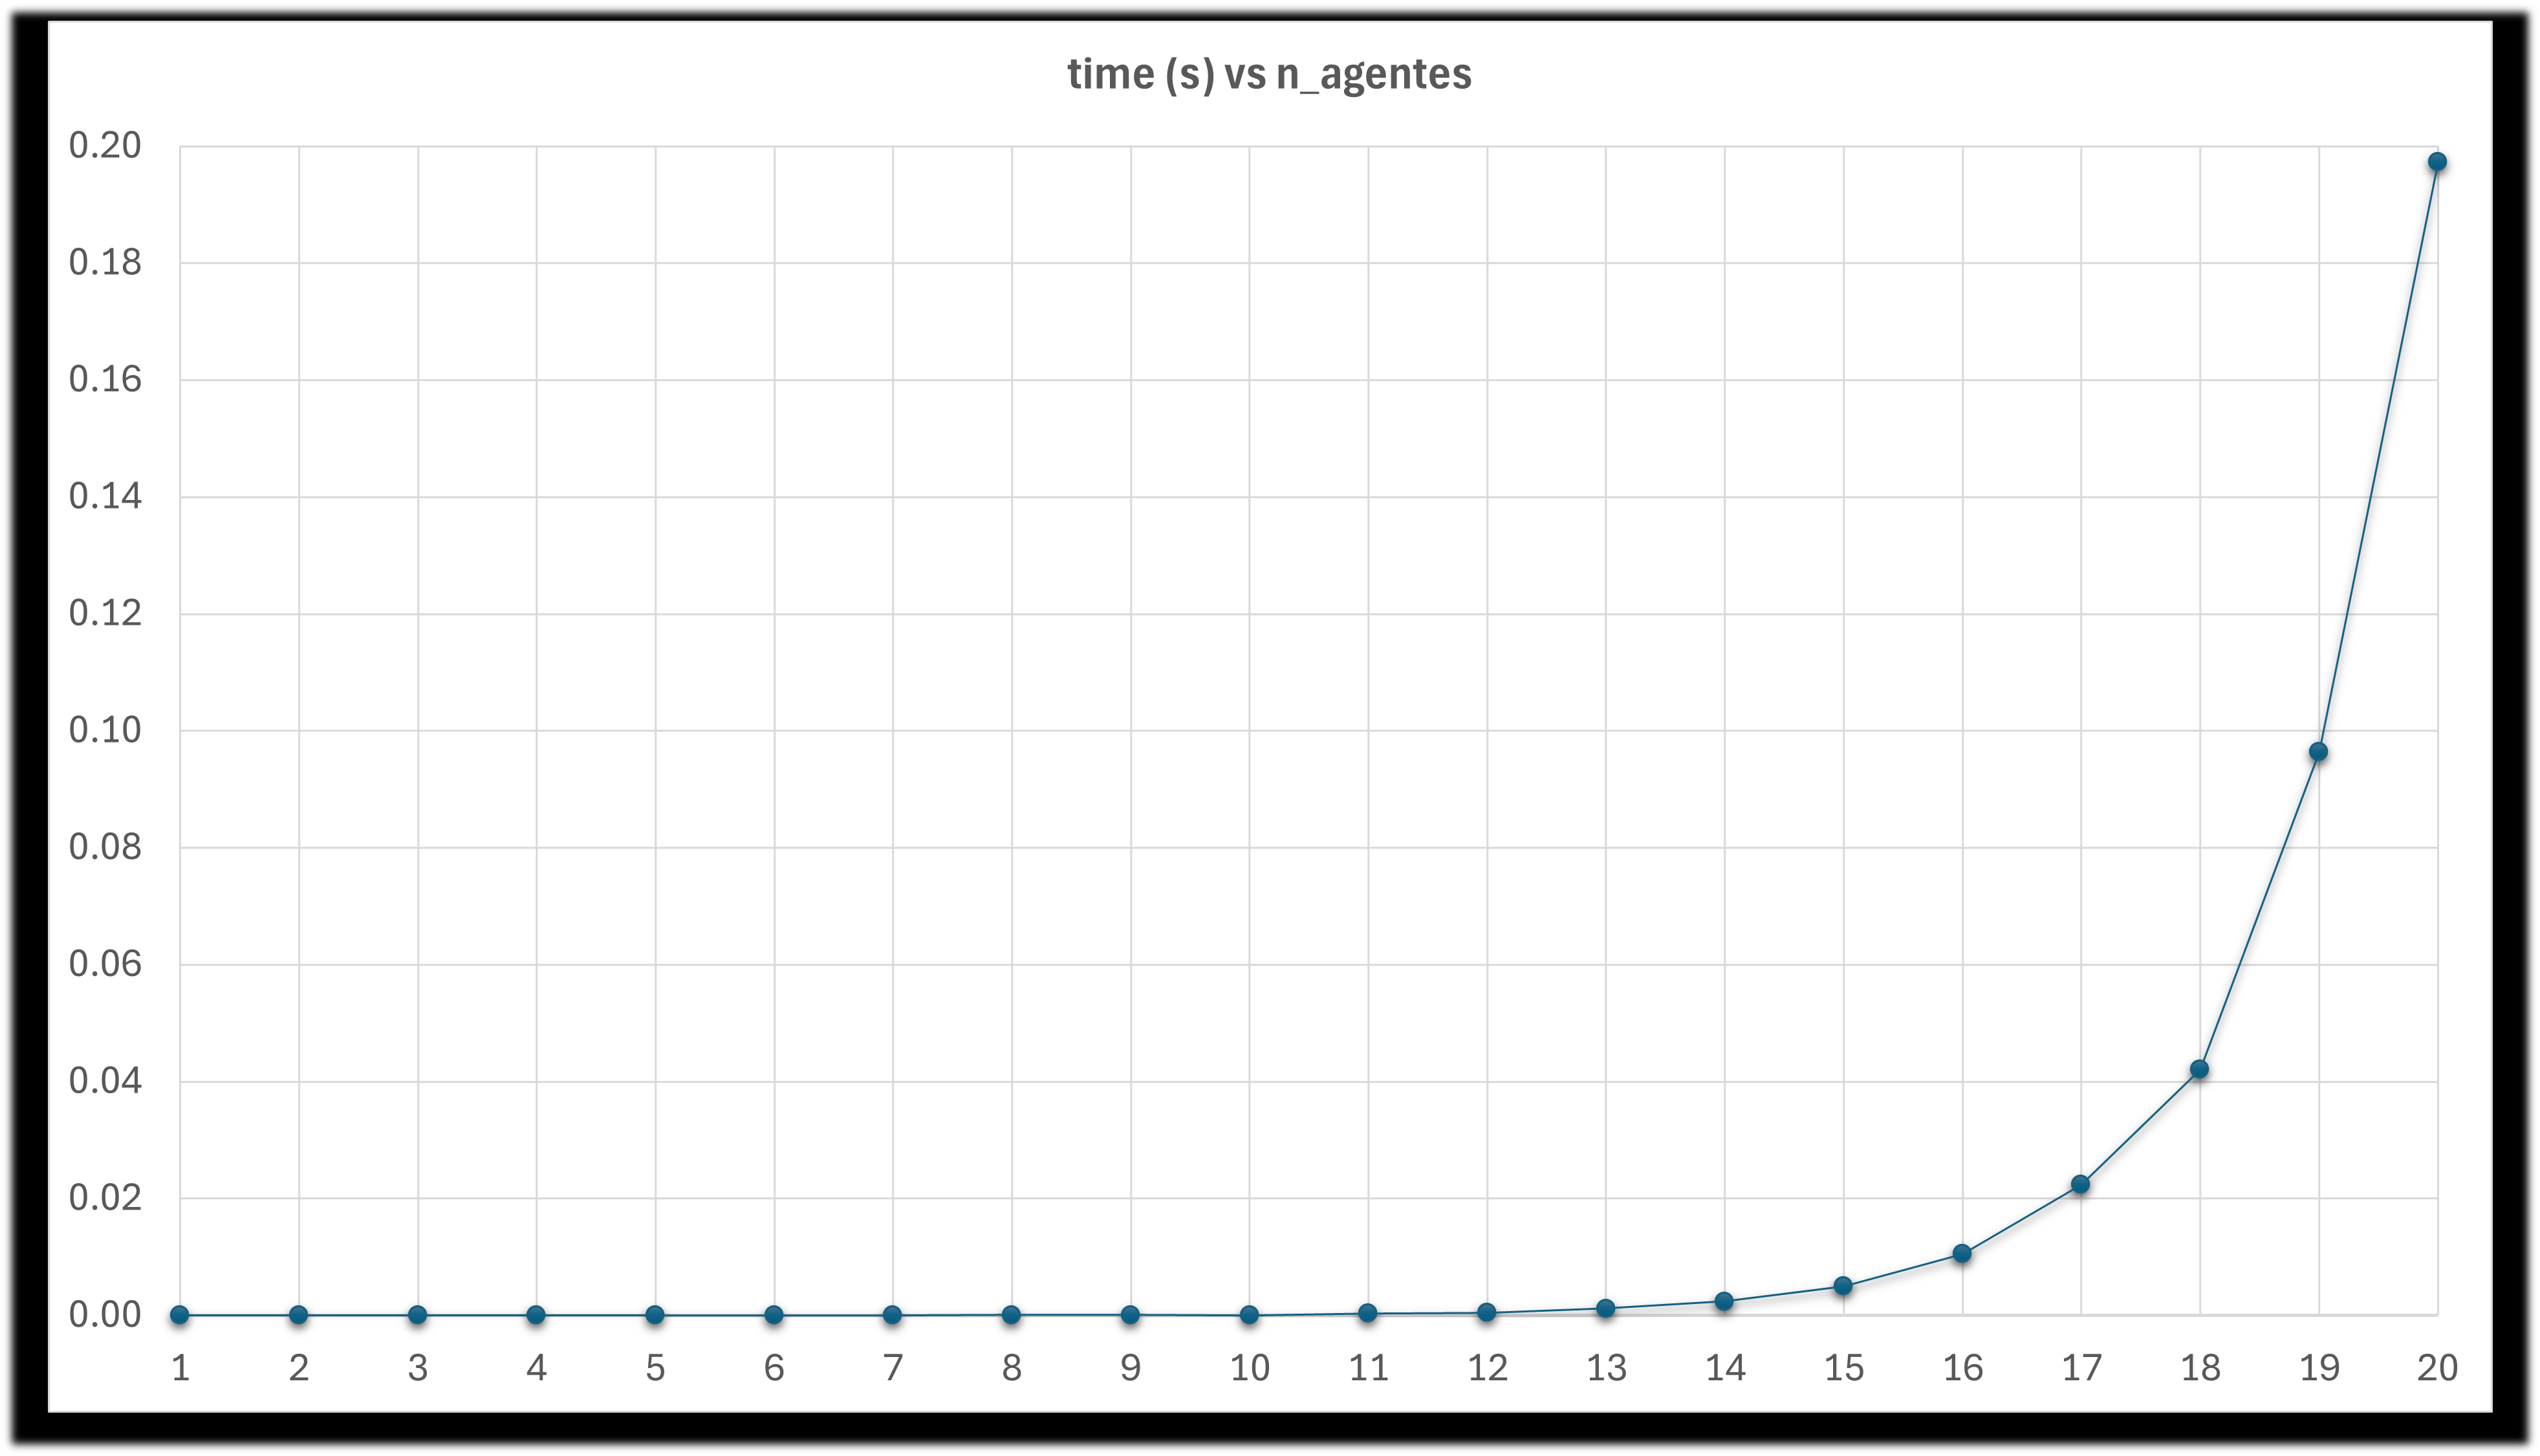
\includegraphics[width=\textwidth]{Images/modexfb1.png}
  \end{minipage}
  \caption{ModexFB exponential} 
  \label{fig:modexfbcomplexity}
\end{figure}

Se puede apreciar claramente la tendencia exponencial de ModexFB en la imagen anterior, donde el tiempo de ejecución aumenta de forma exponencial a medida que se incrementa el número de agentes.

\subsection{Gráfica complejidad  ModexV}
Para comprobar la complejidad del ModexV, como en el anterior caso, realizamos 100 ejecuciones de cada prueba pero esta vez utilizando la batería de pruebas proporcionada. 


\begin{figure}[H]
  \centering
  \begin{minipage}{1\textwidth}
    \centering
    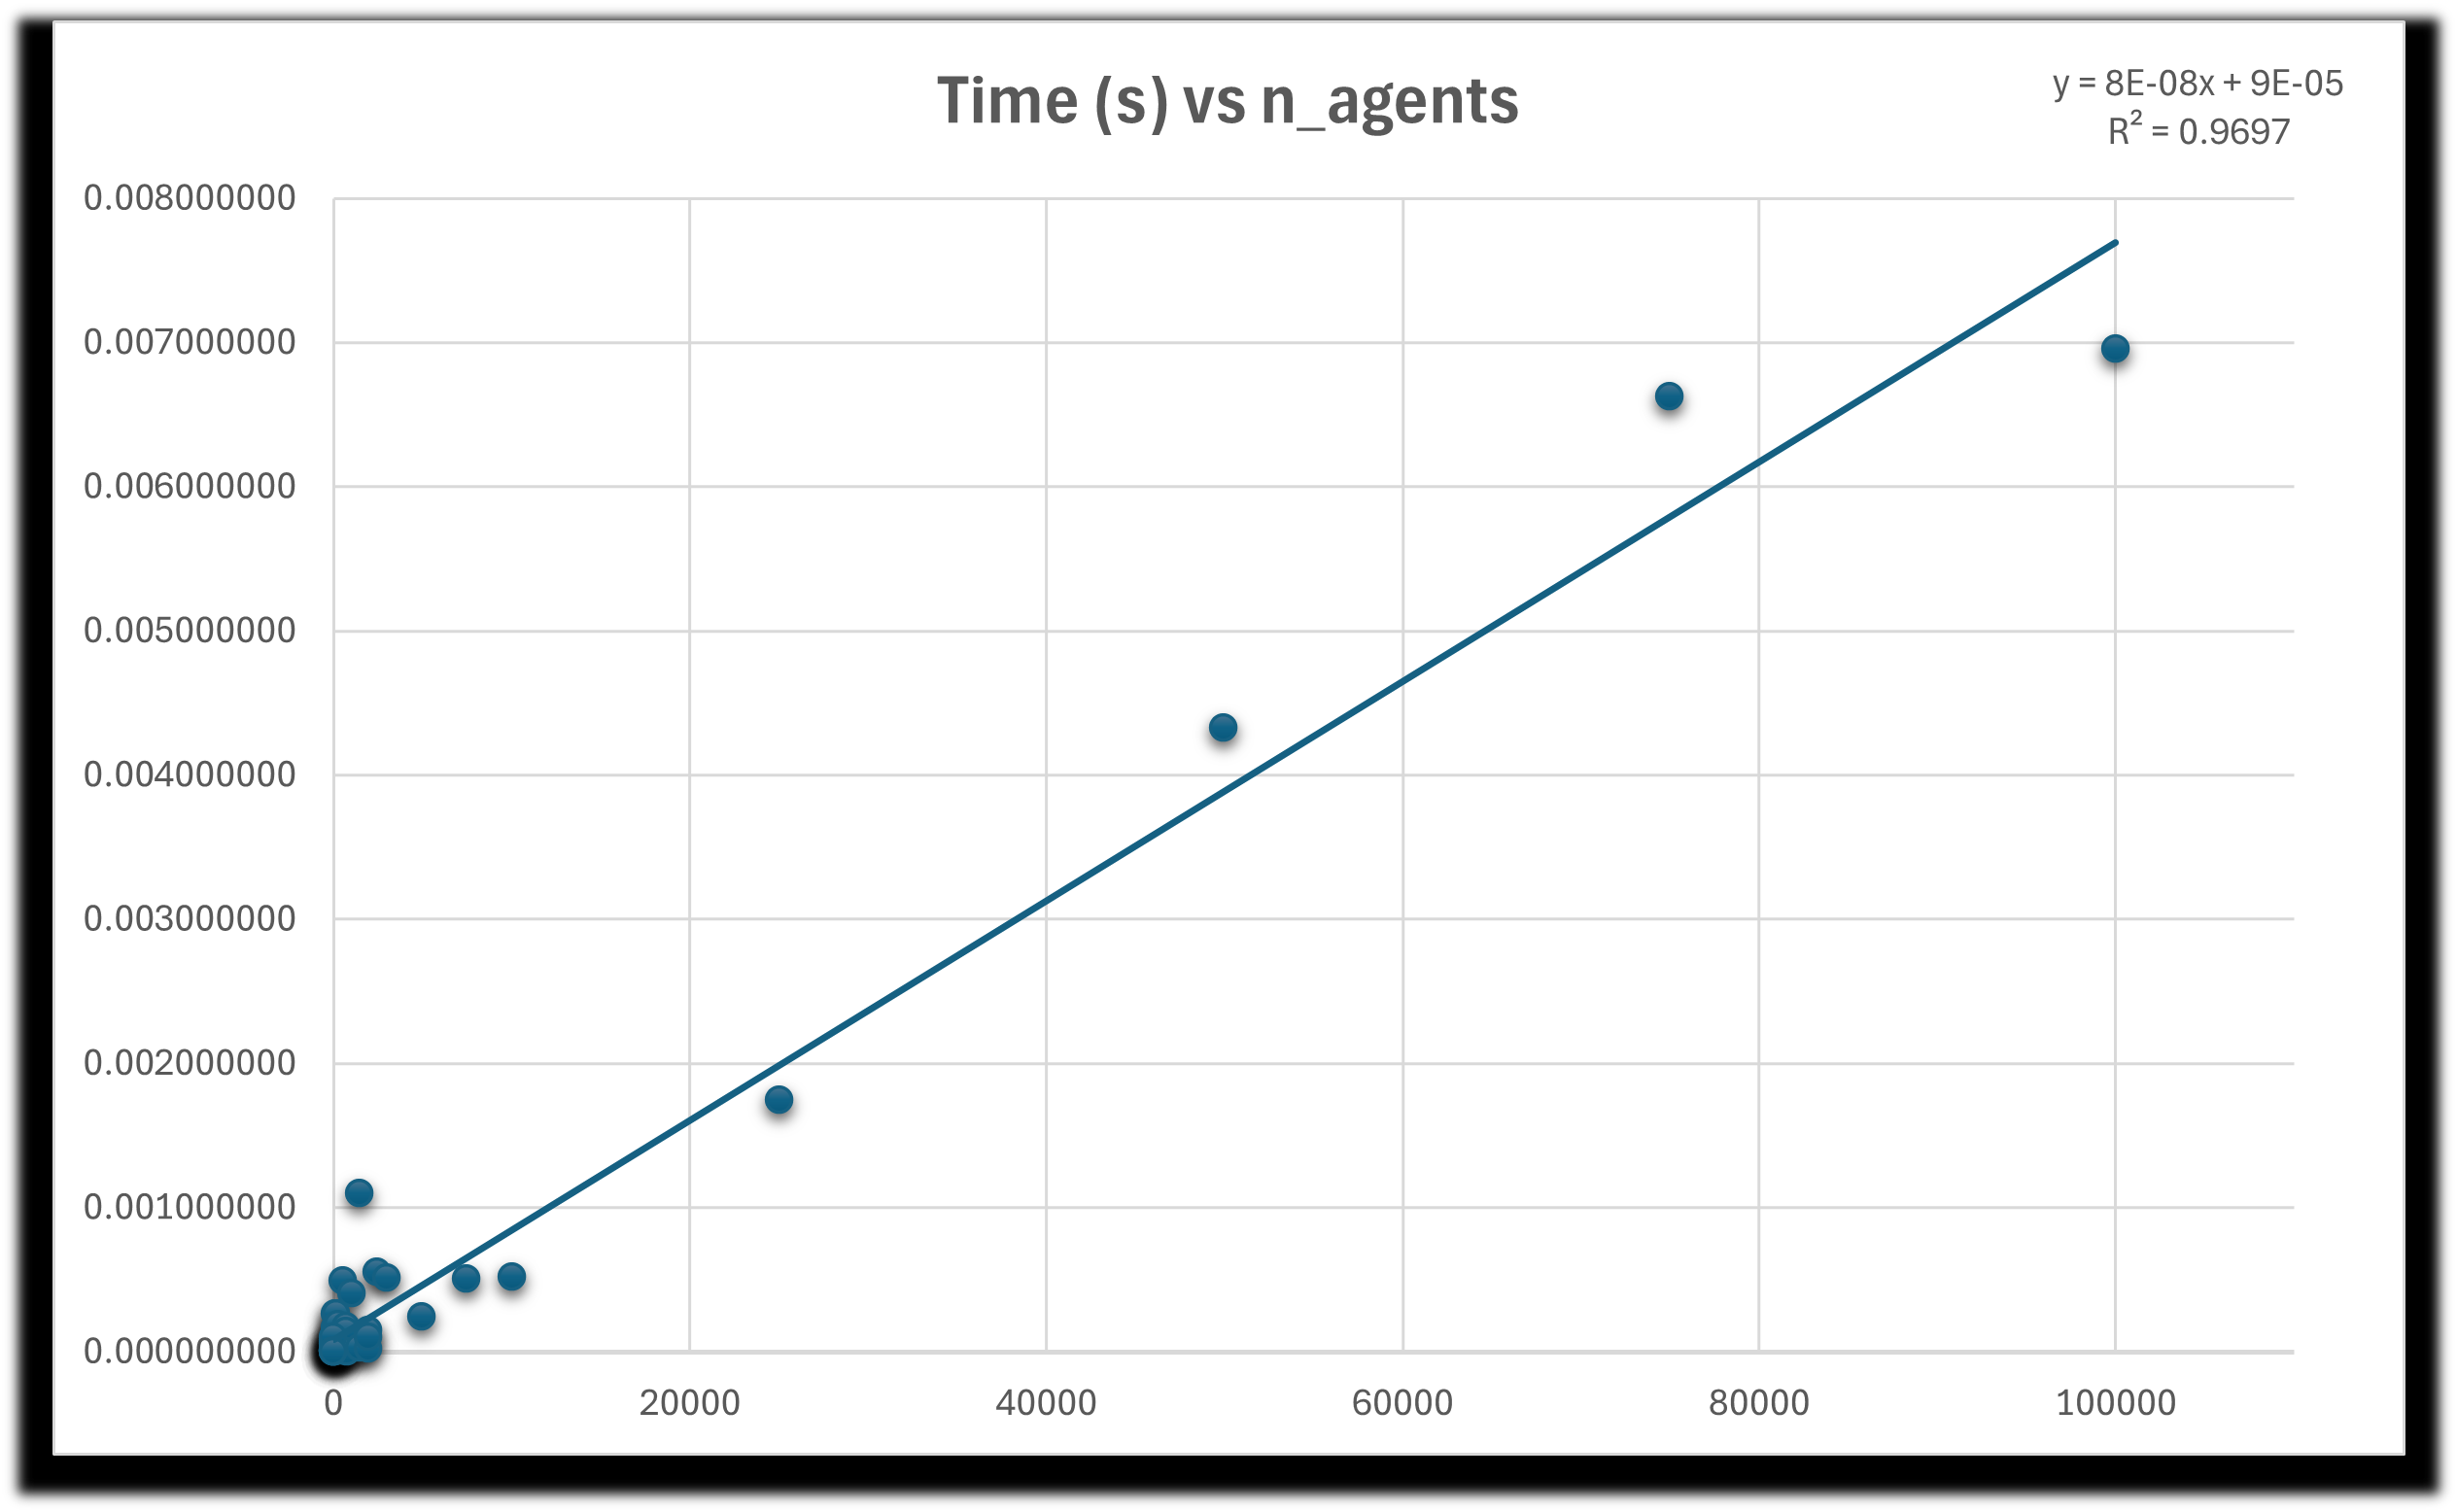
\includegraphics[width=\textwidth]{Images/modexvcomplexity.png}
  \end{minipage}
  \caption{ModexV linear} 
  \label{fig:modexvcomplexity}
\end{figure}
Como se puede apreciar en la anterior gráfica, el tiempo respecto va aumentando la cantidad de agentes se puede ver como una distribución de estos pares denotada por la recta $y=8\cdot 10^{-8}x+9\cdot10^{-5}$.
Comprobando la tendencia a un comportamiento lineal como se dijo anteriormente $\Theta(n)$.


\subsection{Gráfica complejidad ModexPD}
De igualmanera se tomaron 100 pruebas para luego de la misma forma sacar el promedio de tiempos y tener datos bien estructurados basados en la batería dada.

\begin{figure}[H]
  \centering
  \begin{minipage}{1\textwidth}
    \centering
    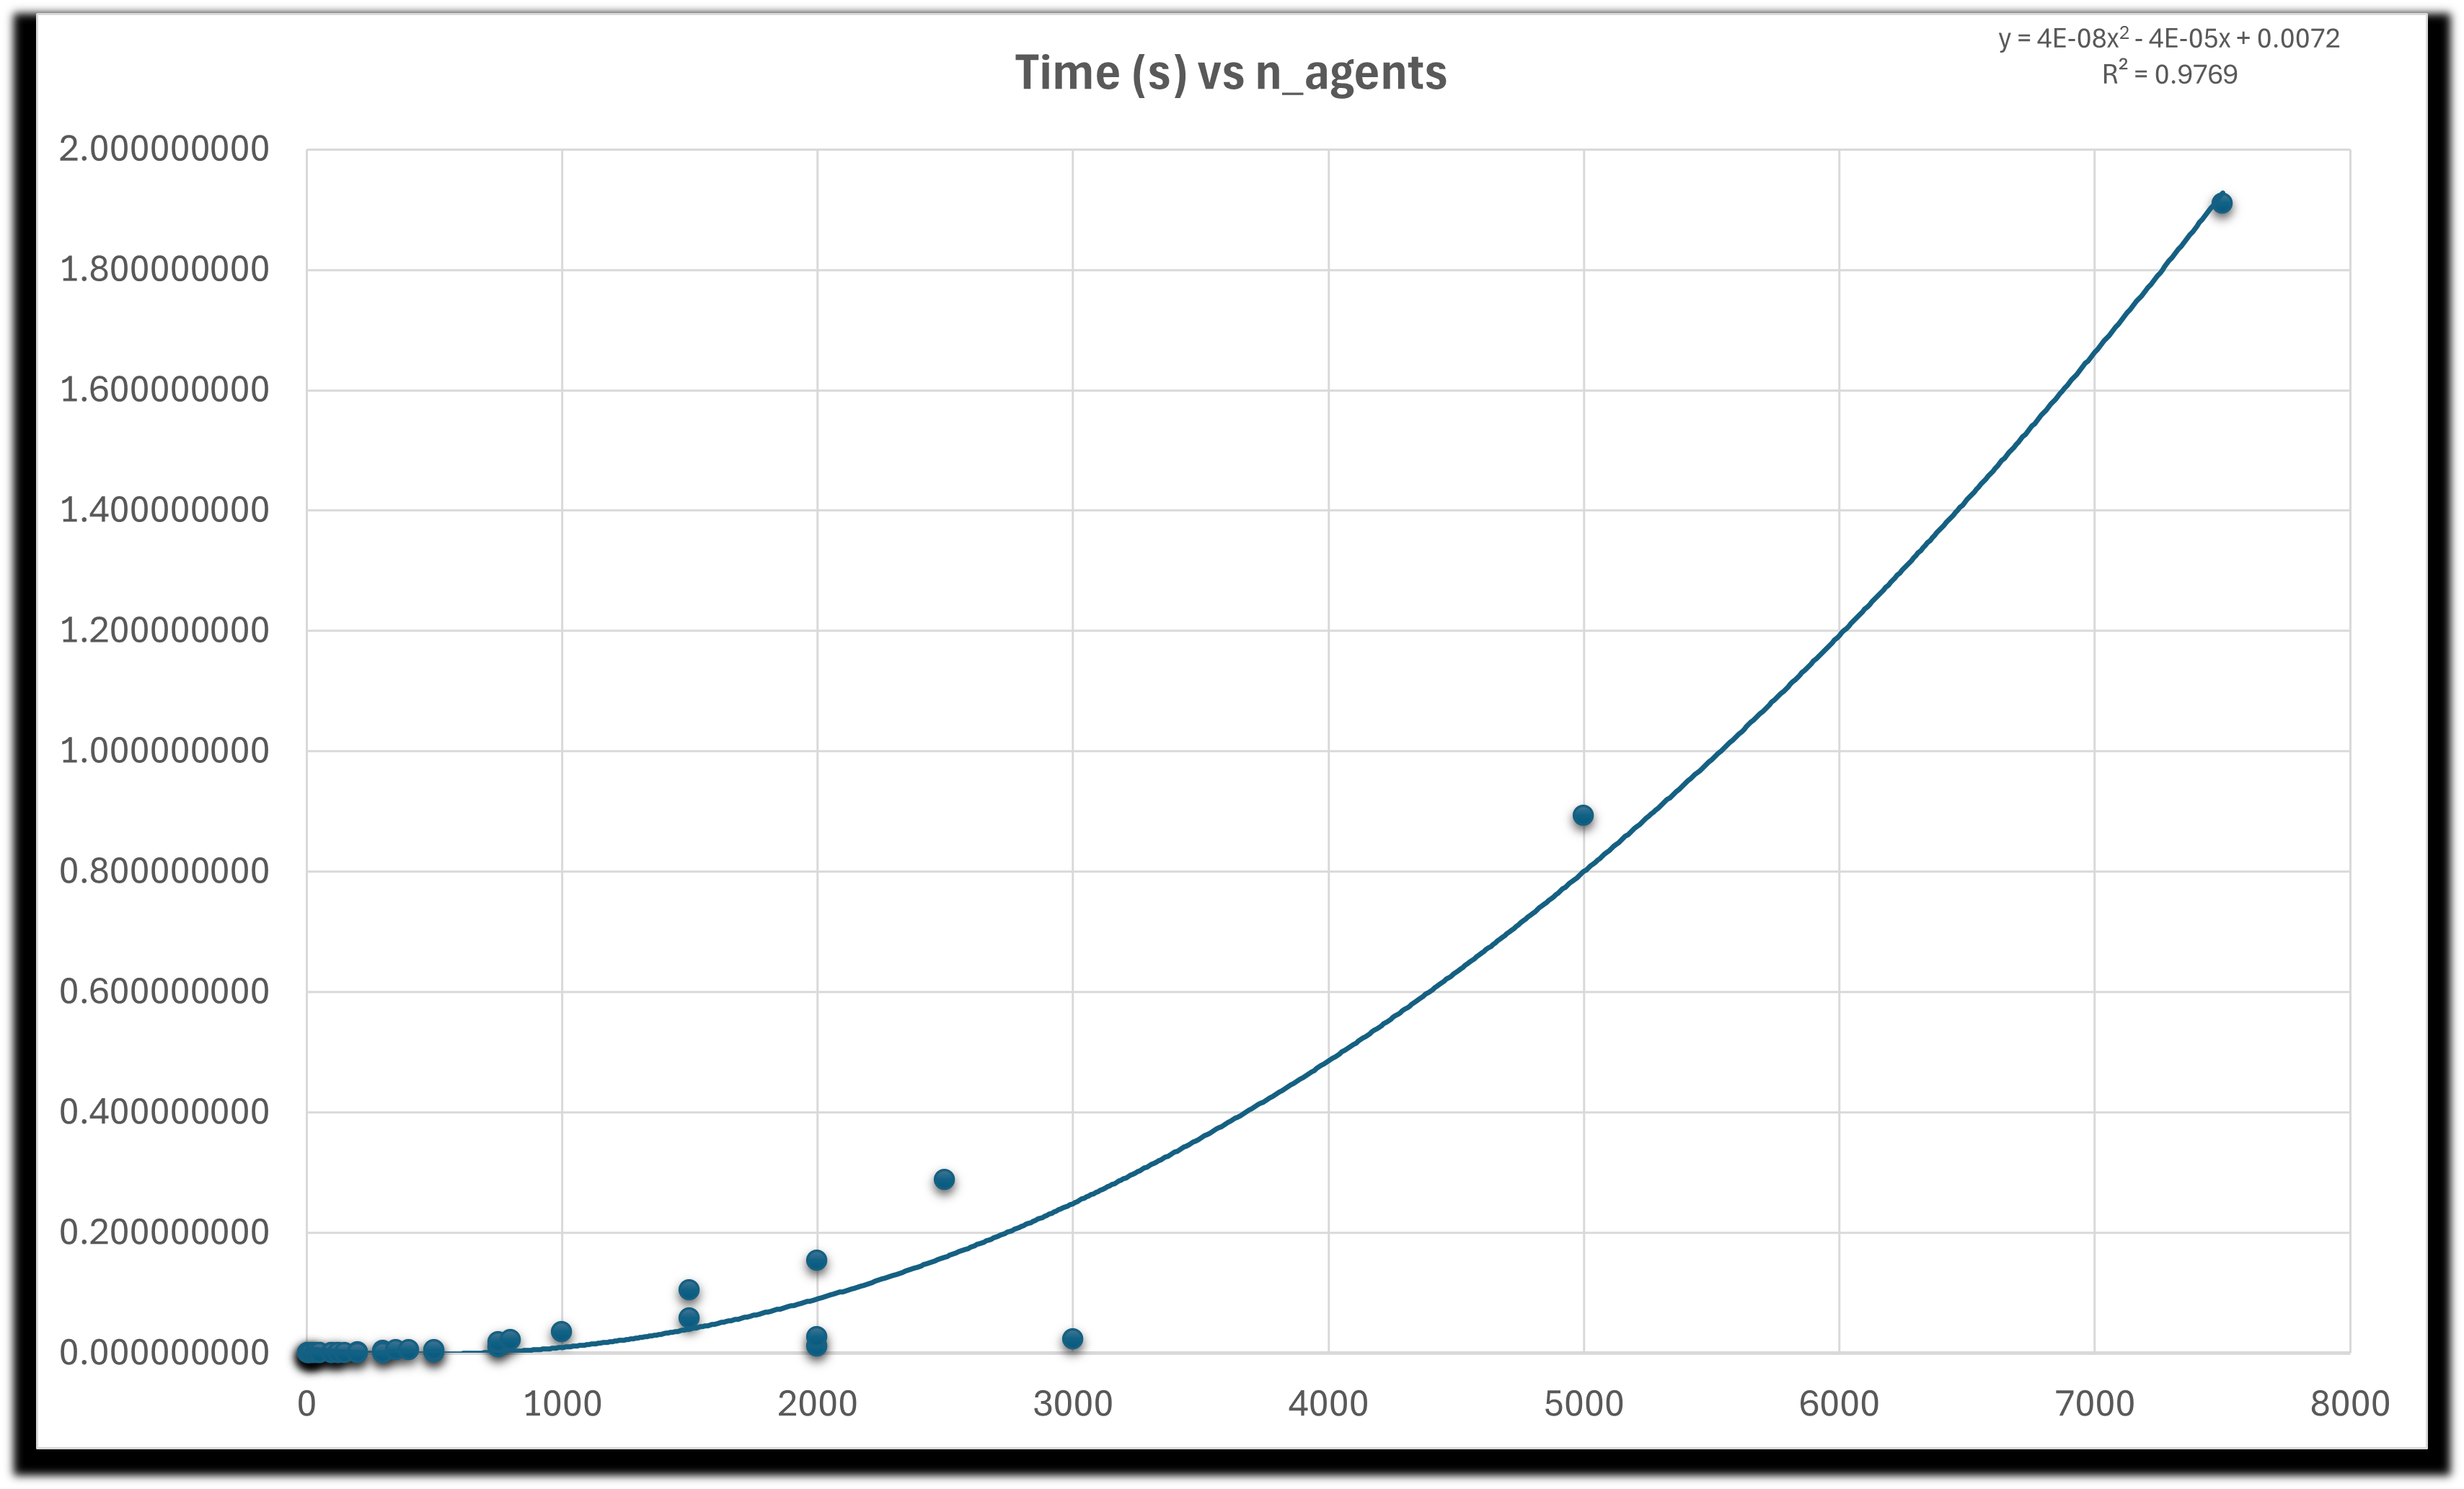
\includegraphics[width=\textwidth]{Images/modexpdcomplexity.png}
  \end{minipage}
  \caption{ModexPD Cuadratic} 
  \label{fig:modexpdcomplexity}
\end{figure}
Se puede apreciar el comportamiento cuadrático de ModexPD en la (\ref{fig:modexpdcomplexity} imagen anterior).

\section{Conclusión}
\label{sec:conclusion}

A partir del análisis realizado de las tres estrategias de diseño implementadas—\textbf{ModexFB} (Fuerza Bruta), \textbf{ModexV} (Voraz) y \textbf{ModexPD} (Programación Dinámica)—se pudieron identificar ventajas y desventajas específicas en cada una, basadas en los datos obtenidos de las pruebas ejecutadas.

\subsection{Ventajas y Desventajas de ModexFB}

La principal ventaja de la estrategia \textbf{ModexFB} radica en su capacidad para encontrar la solución óptima en todos los casos, garantizando la correctitud del resultado. Esto se debe a que evalúa todas las posibles combinaciones de agentes y recursos, asegurando que no se omita ninguna solución potencialmente mejor.

Sin embargo, su desventaja más significativa es su complejidad temporal exponencial $O(2^n)$, lo que la hace impracticable para problemas con un número moderado a grande de agentes. Como se observó en las pruebas, después de la prueba 6, el algoritmo no pudo completarse debido a limitaciones de memoria, ya que requería más recursos de los disponibles (más de 128 GB de RAM). Esto limita su uso a casos muy pequeños y lo hace ineficiente en la práctica para problemas de tamaño real.

\subsection{Ventajas y Desventajas de ModexV}

La estrategia \textbf{ModexV} presenta como principal ventaja su rapidez y eficiencia en términos de tiempo de ejecución. Con una complejidad lineal $\Theta(n)$, es capaz de manejar grandes cantidades de agentes sin un incremento significativo en el tiempo de procesamiento, como se evidenció en las pruebas realizadas donde los tiempos fueron generalmente inferiores a una milésima de segundo.

No obstante, su desventaja radica en que no garantiza la obtención de la solución óptima. Aunque en las pruebas realizadas las diferencias con la solución óptima fueron mínimas (en promedio, una variación porcentual de 0.2898\%), hubo casos en los que no se alcanzó el valor correcto de la solución. Esto implica que, si bien es una buena aproximación y puede ser útil cuando se requiere rapidez, no es recomendable en situaciones donde la exactitud del resultado es crítica.

\subsection{Ventajas y Desventajas de ModexPD}

La estrategia \textbf{ModexPD} combina algunas de las ventajas de las dos anteriores. Por un lado, garantiza la correctitud de la solución, al igual que \textbf{ModexFB}. Por otro lado, es más eficiente que la fuerza bruta, ya que su complejidad es cuadrática $O(n^2)$, lo que permite manejar problemas de tamaño moderado con tiempos de ejecución aceptables.

Sin embargo, su desventaja se manifiesta en problemas de gran escala. Al igual que con la fuerza bruta, \textbf{ModexPD} también enfrentó limitaciones de memoria en pruebas más allá de la número 36, donde se requería más de 128 GB de RAM para su ejecución. Esto limita su aplicabilidad en problemas muy grandes, donde los recursos computacionales necesarios superan las capacidades habituales.
\subsection{Lenguaje de programación escogido}

Algo muy importante a recalcar es el lenguaje de programación, en nuestro caso utilizamos (\href{https://go.dev/}{Go}) un lenguaje compilado que es muy útil para algoritmos con alta complejidad temporal, en este caso progrmación dinámica o algoritmos de búsqueda y cálculos combinatorios, por ejemplo.

Una de las limitantes que vimos fue la falta de memoria, pero esto no se debió al lenguaje de programación, sino a la capacidad de la máquina en la que se ejecutaba el programa. En este caso, se utilizó una máquina con 32 GB de RAM y capacidad de 128 GB de \textit{swap}, lo que limitó la cantidad de agentes que se podían manejar en las pruebas. Sin embargo, el lenguaje de programación en sí no presentó problemas de rendimiento y permitió implementar los algoritmos de manera eficiente y sencilla. De hecho estamos conformes con todos los tiempos de ejecución obtenidos ya que no fueron significativamente altos y se pudieron manejar sin problemas.
\subsection{Recomendaciones}

En función de las ventajas y desventajas identificadas, se puede concluir que:

Para problemas de pequeña escala, donde el número de agentes es reducido, \textbf{ModexFB} es una opción viable si se busca obtener la solución óptima sin importar el tiempo de ejecución.

Para problemas de gran escala, donde la rapidez es esencial y una aproximación cercana a la óptima es aceptable, \textbf{ModexV} es la estrategia más adecuada debido a su eficiencia temporal.

Para problemas de tamaño moderado, donde se requiere exactitud pero el número de agentes no es excesivamente grande, \textbf{ModexPD} ofrece un equilibrio entre eficiencia y correctitud.

Es importante considerar las limitaciones de cada estrategia en función de los recursos disponibles y los requisitos específicos del problema a resolver. La elección de la estrategia debe basarse en un balance entre la necesidad de precisión y la eficiencia computacional.
\end{document}